\subsection*{Supplementary figures for the house sparrow study}

We include figures containing the estimated relative importance of all covariates, and $R^2$ estimates, from both integration strategies used in the house sparrow study (\Cref{sec:heritability_method}). The figures are presented in the same order as in the main text, starting with the body mass model, followed by the wing length model, and finally the tarsus length model.
\\
\\
The posterior distribution of relative importance of the fixed effects (\Cref{fig:mass_fixed_sparrows}) show that they are mostly very small. The covariates \textit{FGRM, age} and \textit{other} seem to have been allocated no importance at all, with the distributions of \textit{FGRM} and \textit{other} following a negative exponential pattern. Recall that importance calculations include squaring the coefficients, and so no negative importance can be allocated to a covariate. Therefore, the sharp decay from zero seems reasonable. The covariates \textit{month, sex} and \textit{outer} seem to have been allocated a small share of the importance, with \textit{month} and \textit{sex} showing signs of a normal distribution.
\begin{figure}[H]%\ContinuedFloat
  \centering
  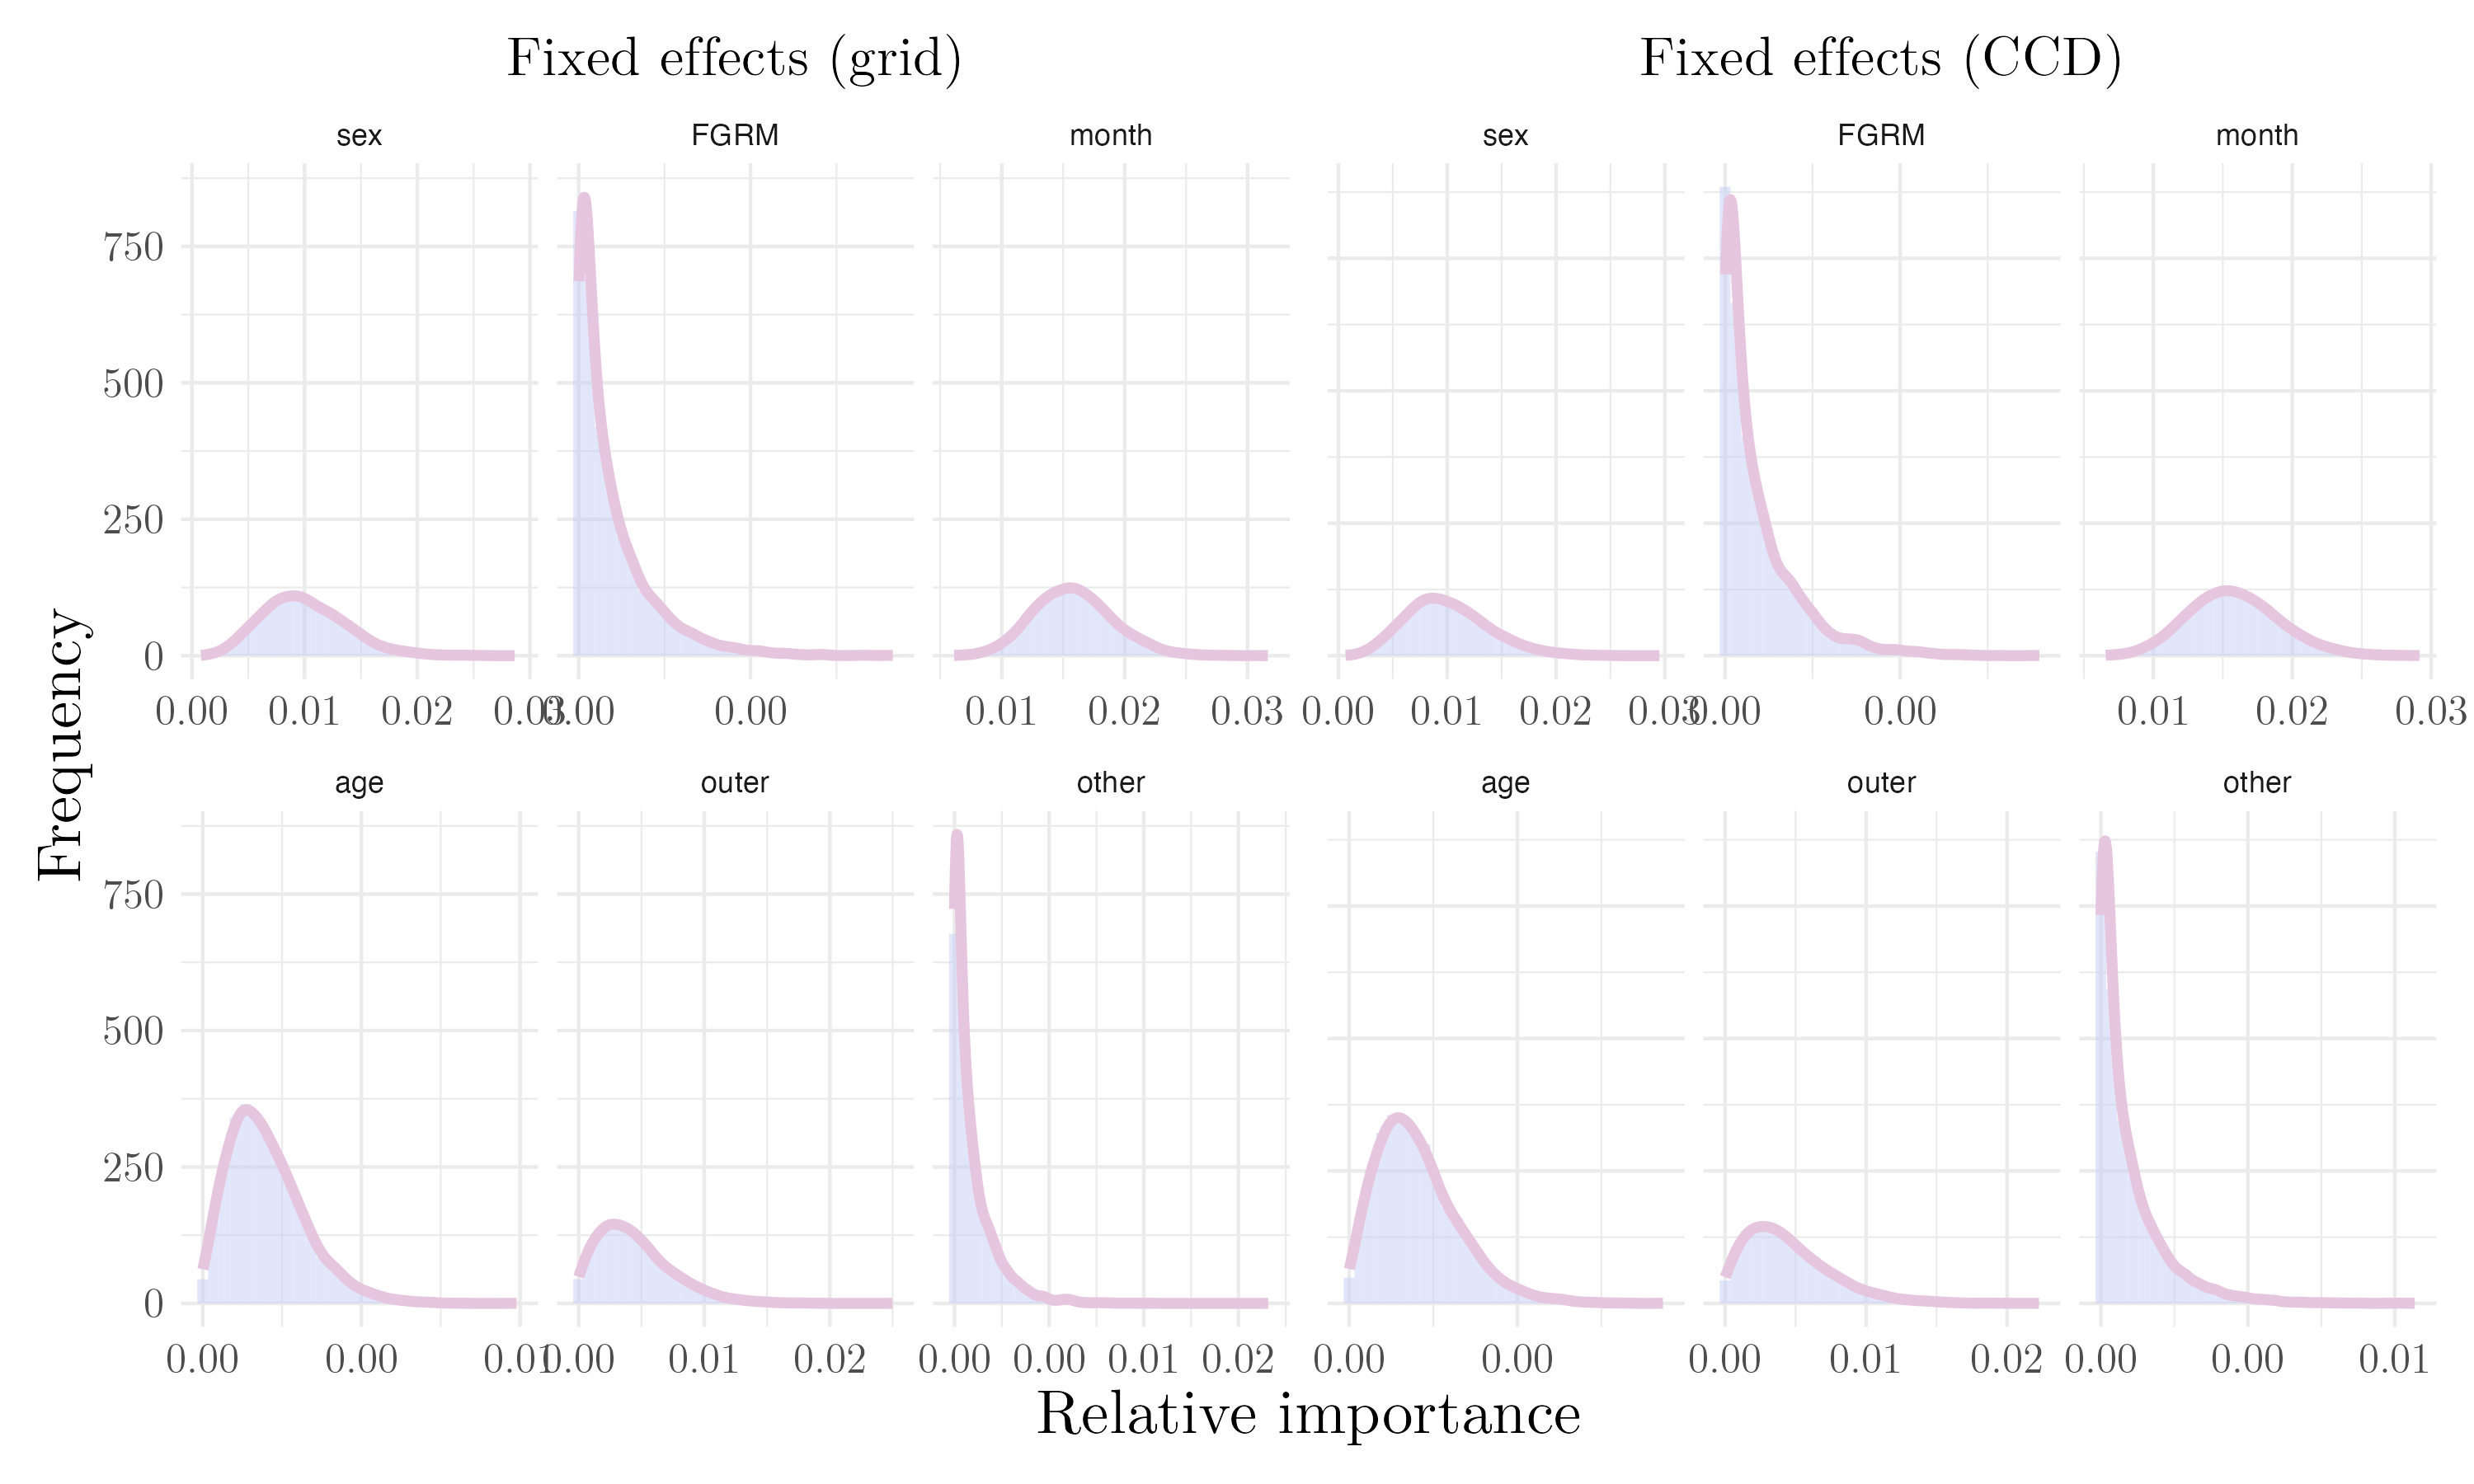
\includegraphics[width=1\linewidth]{Figures/House sparrow study/Mass_fixed.png}
  \caption[Posterior relative importance distributions of all fixed effects in body mass model for house sparrow study]{Posterior relative importance distributions of all fixed effects in heritability of body mass model for house sparrow study. The grid integration is displayed on the left, and CCD on the right.}
  \label{fig:mass_fixed_sparrows}
\end{figure}

\begin{figure}[H]%\ContinuedFloat
  \centering
  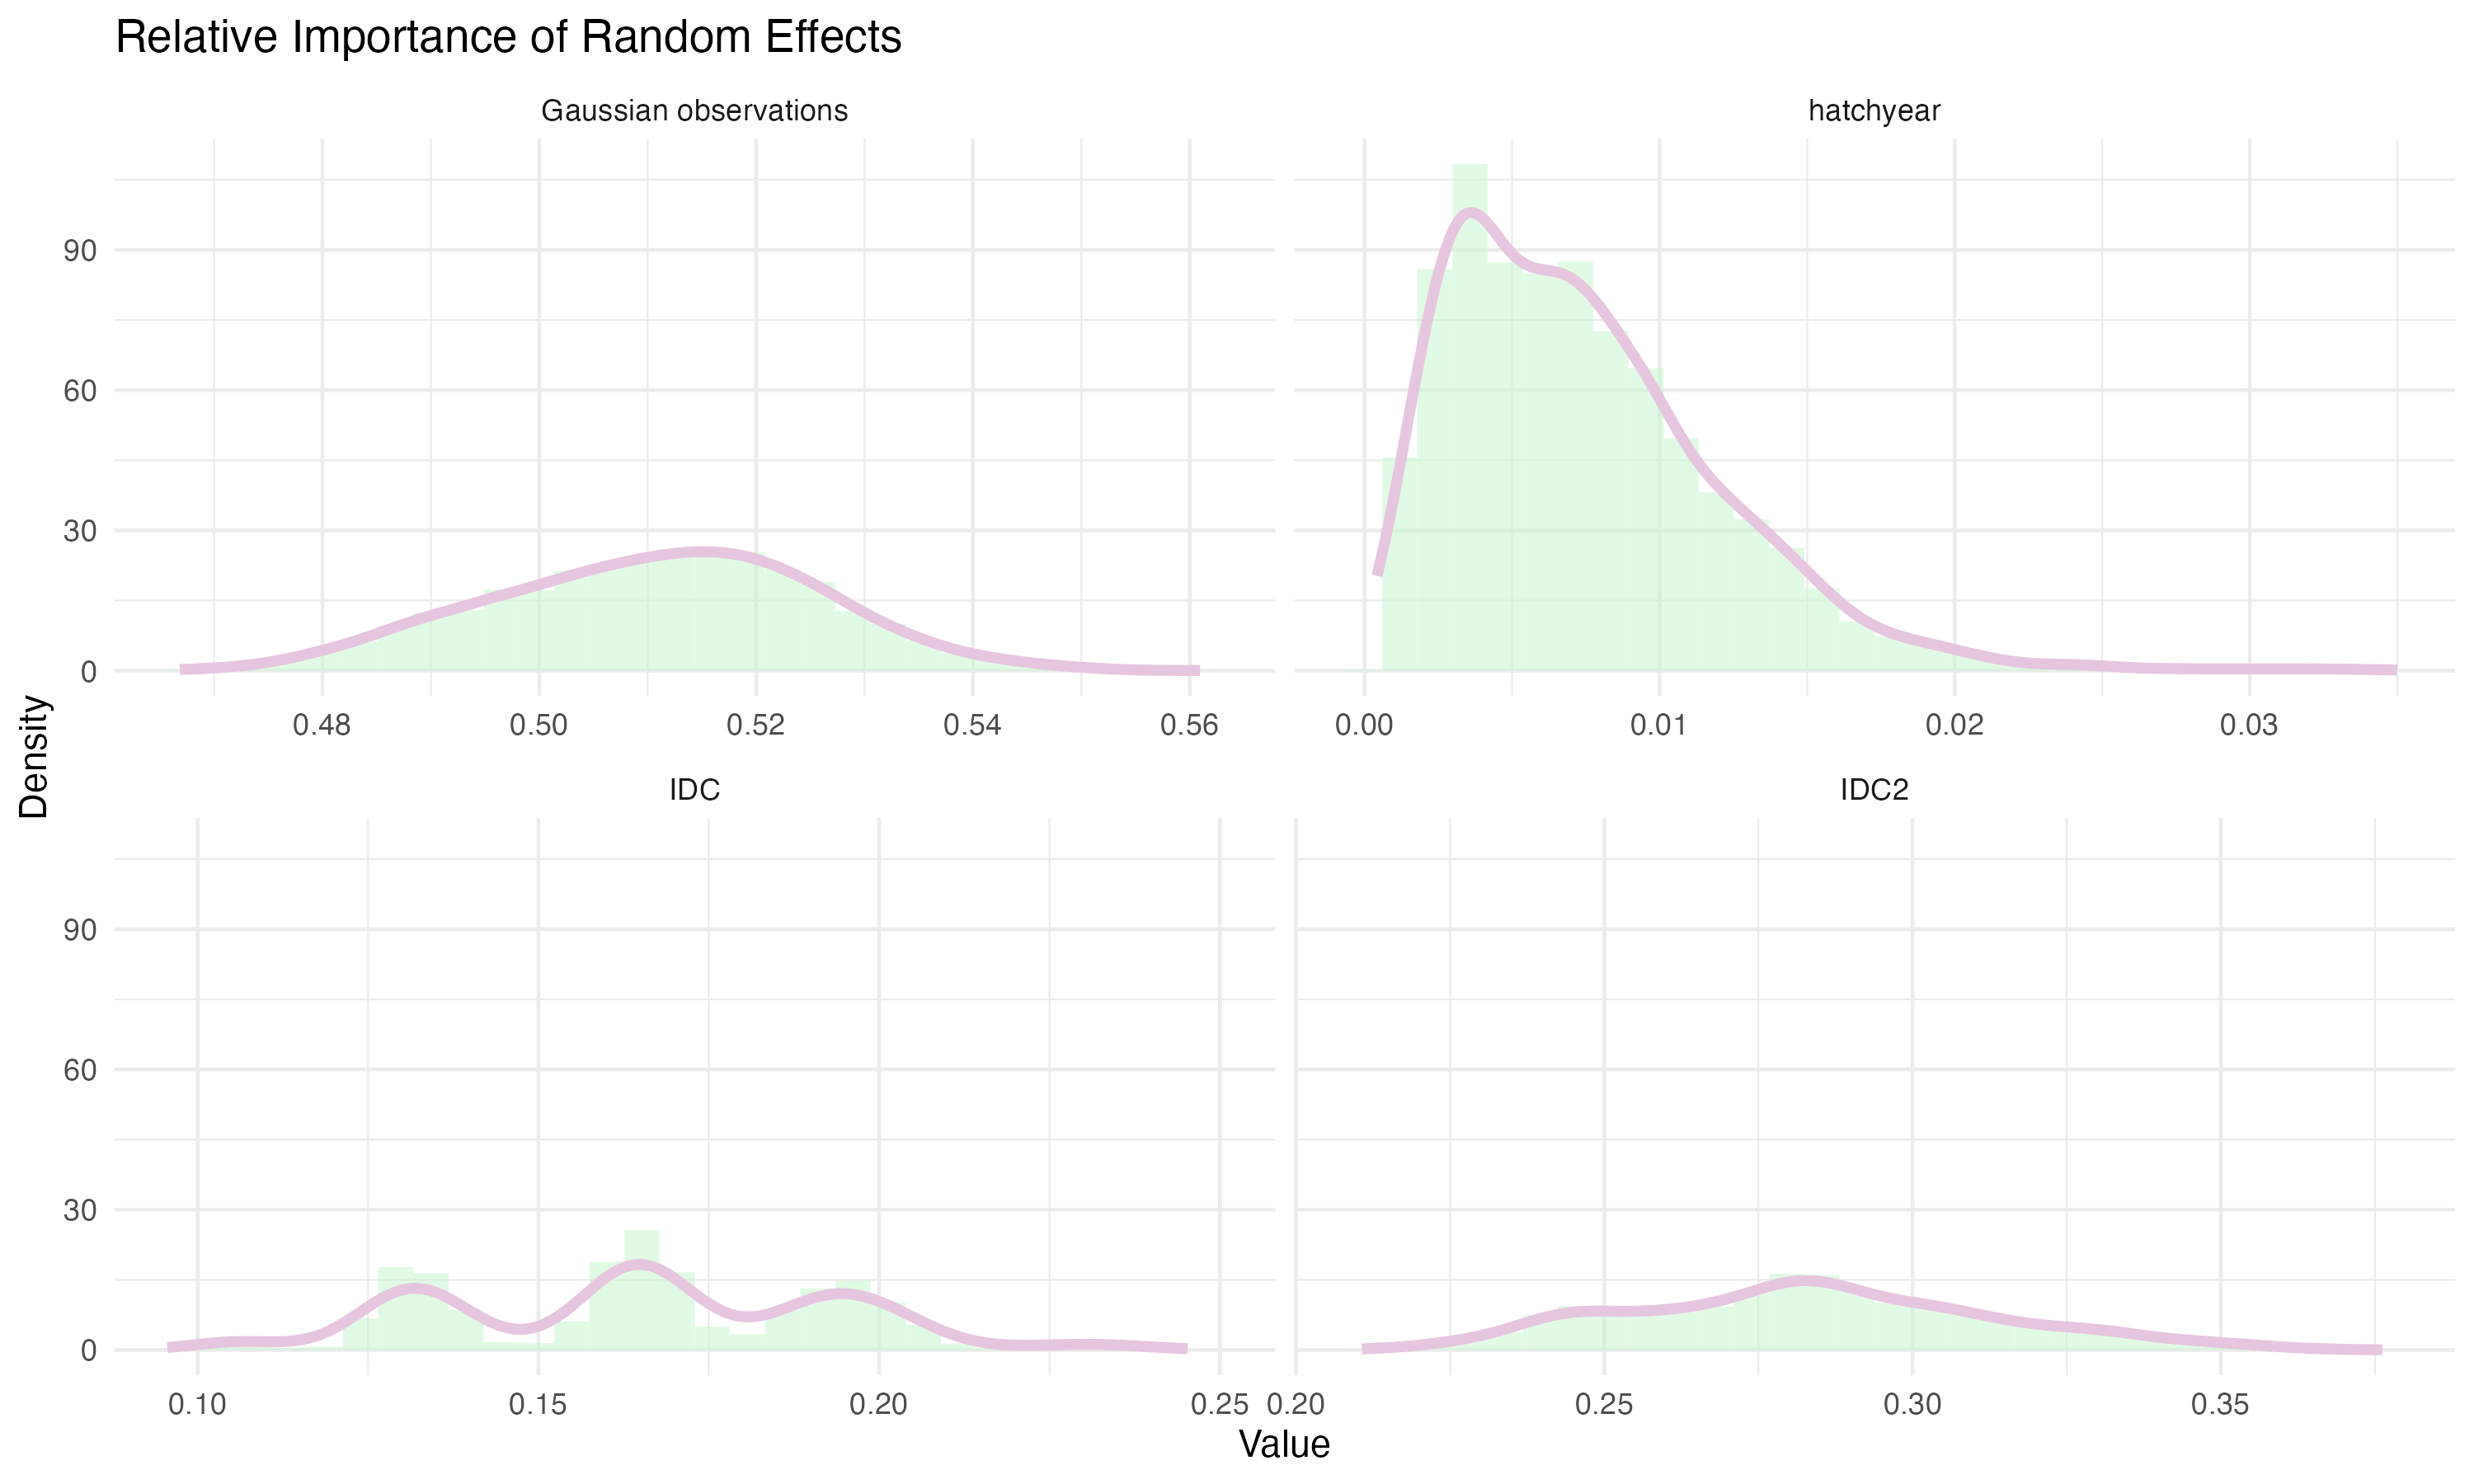
\includegraphics[width=1\linewidth]{Figures/House sparrow study/Mass_random.png}
  \caption[Posterior relative importance distributions of all random effects in body mass model for house sparrow study]{Posterior relative importance distributions of all random effects in heritability of body mass model for house sparrow study. The grid integration is displayed on the left, and CCD on the right.}
  \label{fig:mass_random_sparrows}
\end{figure}

\begin{figure}[H]%\ContinuedFloat
  \centering
  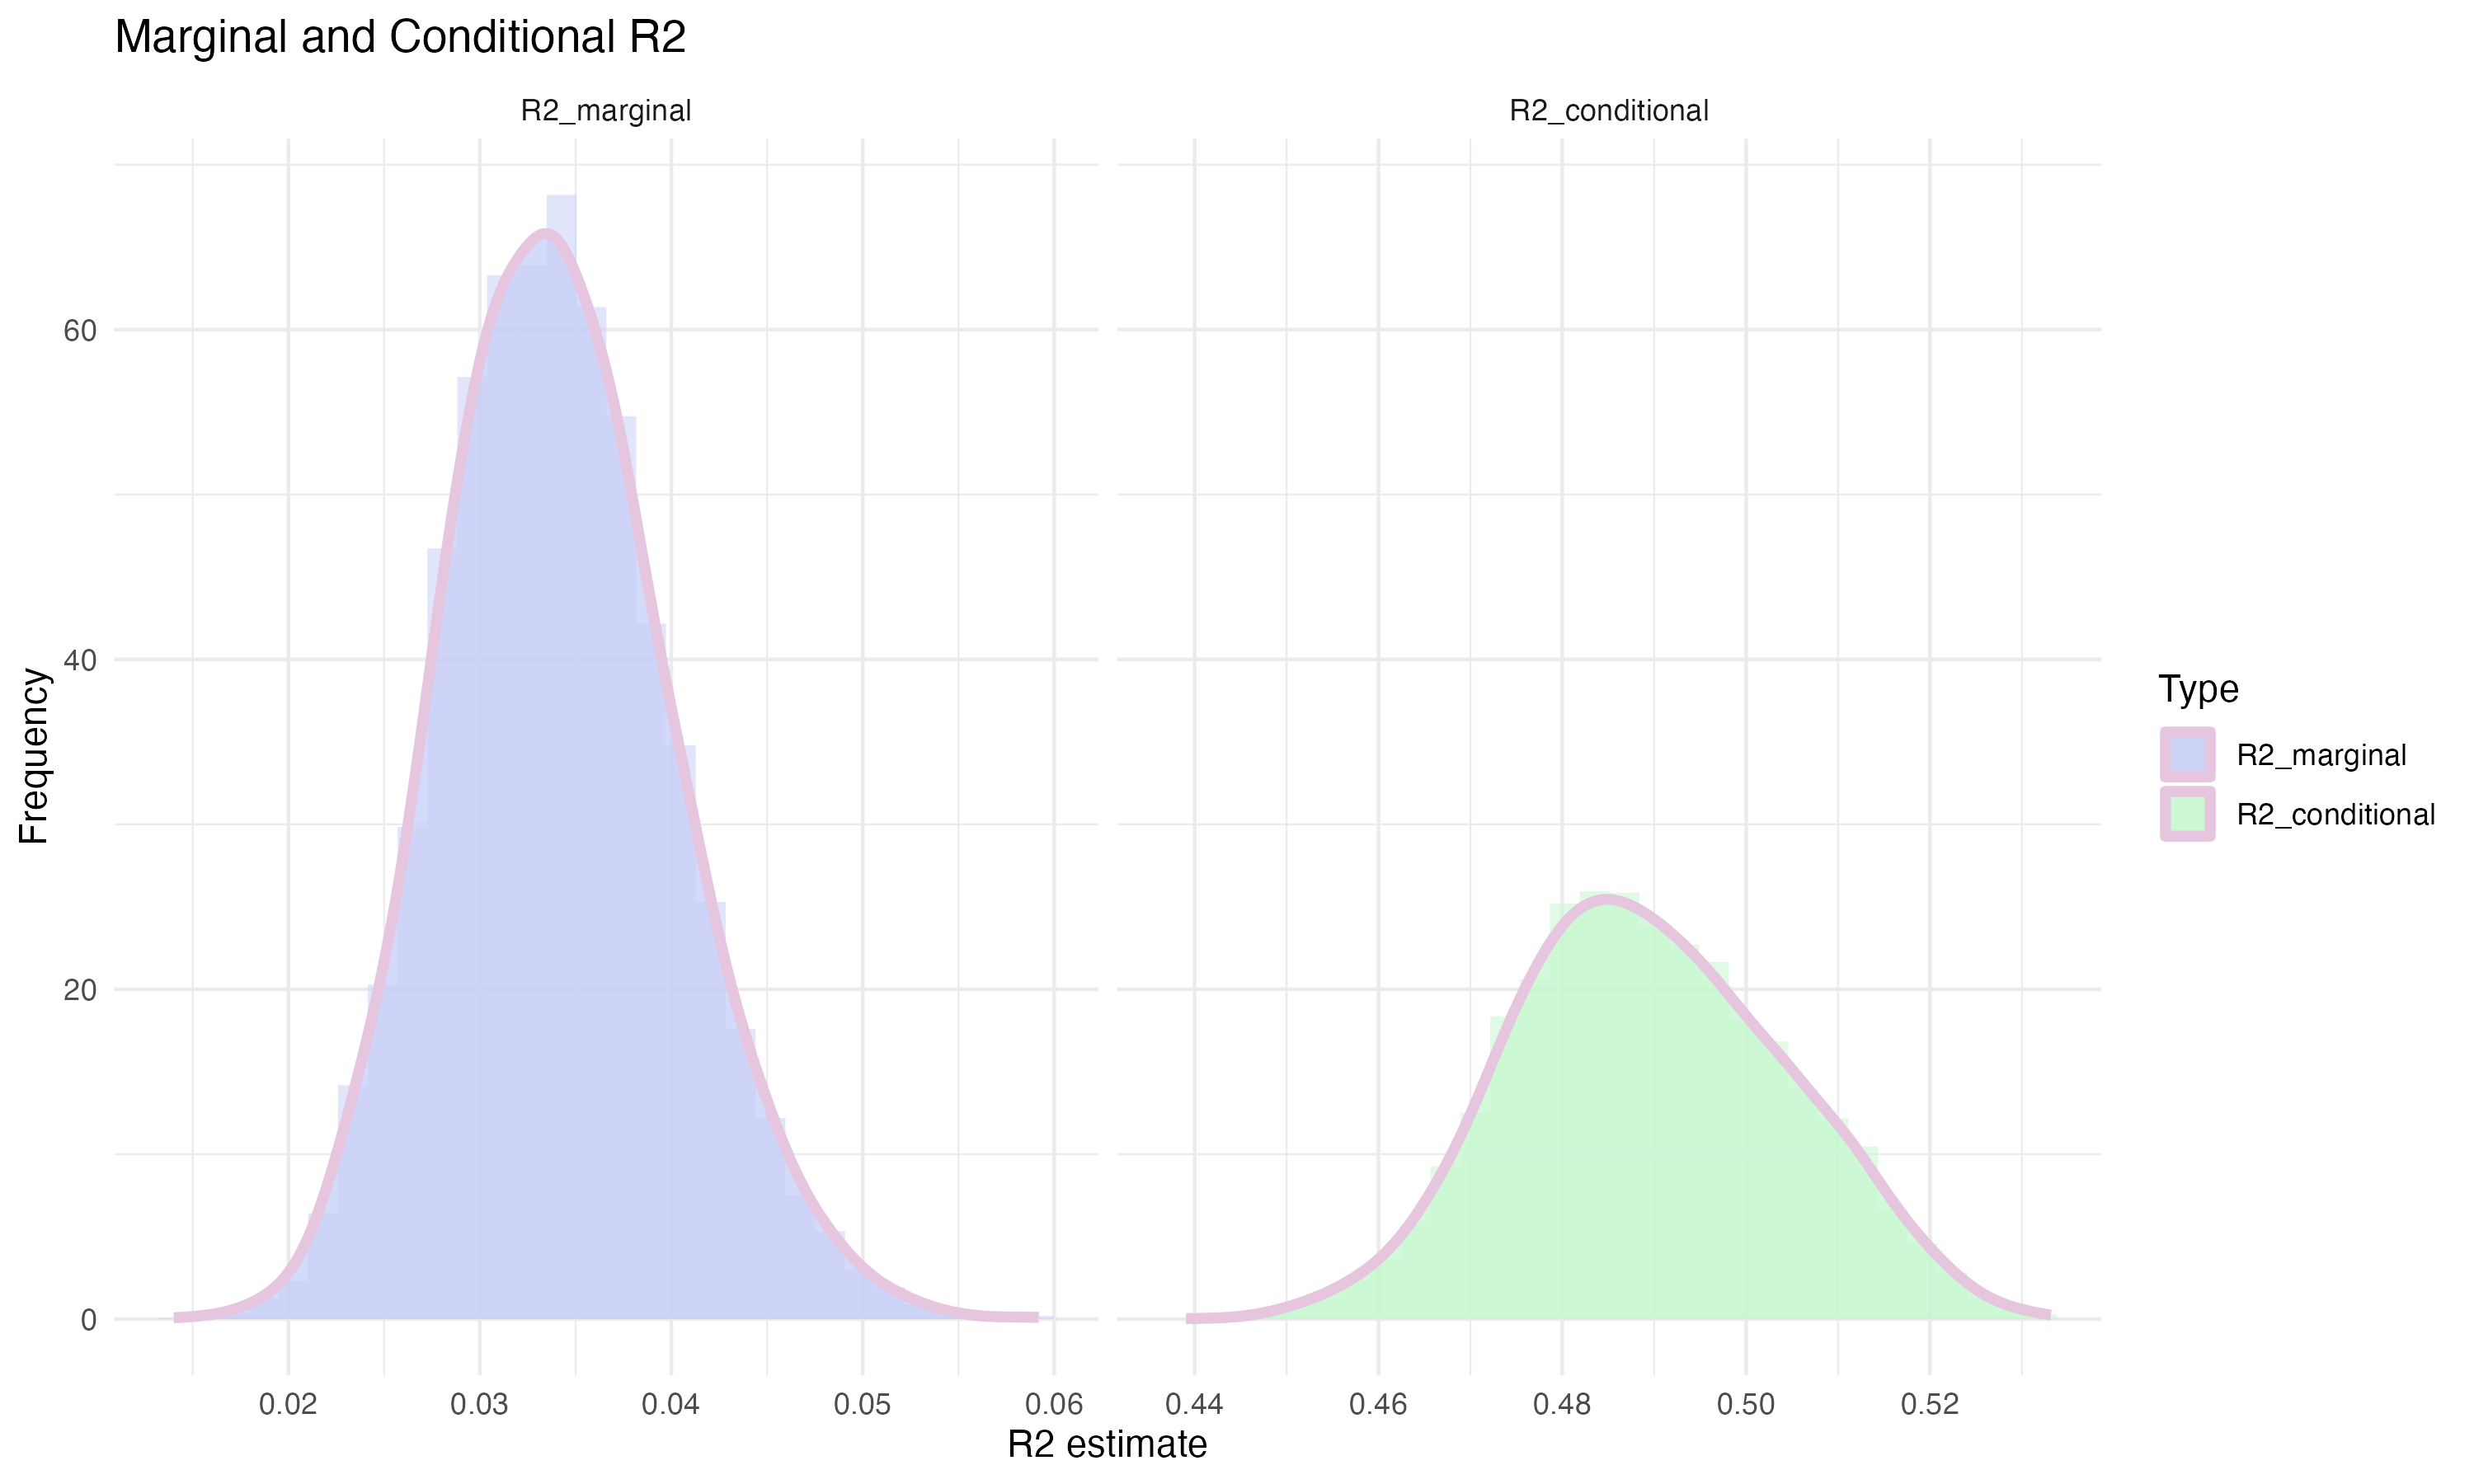
\includegraphics[width=1\linewidth]{Figures/House sparrow study/Mass_r2.png}
  \caption[Posterior distributions of $R^2$ values in body mass model for house sparrow study]{Posterior distributions of $R^2$ values in heritability of body mass model for house sparrow study. The grid integration is displayed on the left, and CCD on the right.}
  \label{fig:mass_r2}
\end{figure}

\begin{figure}[H]%\ContinuedFloat
  \centering
  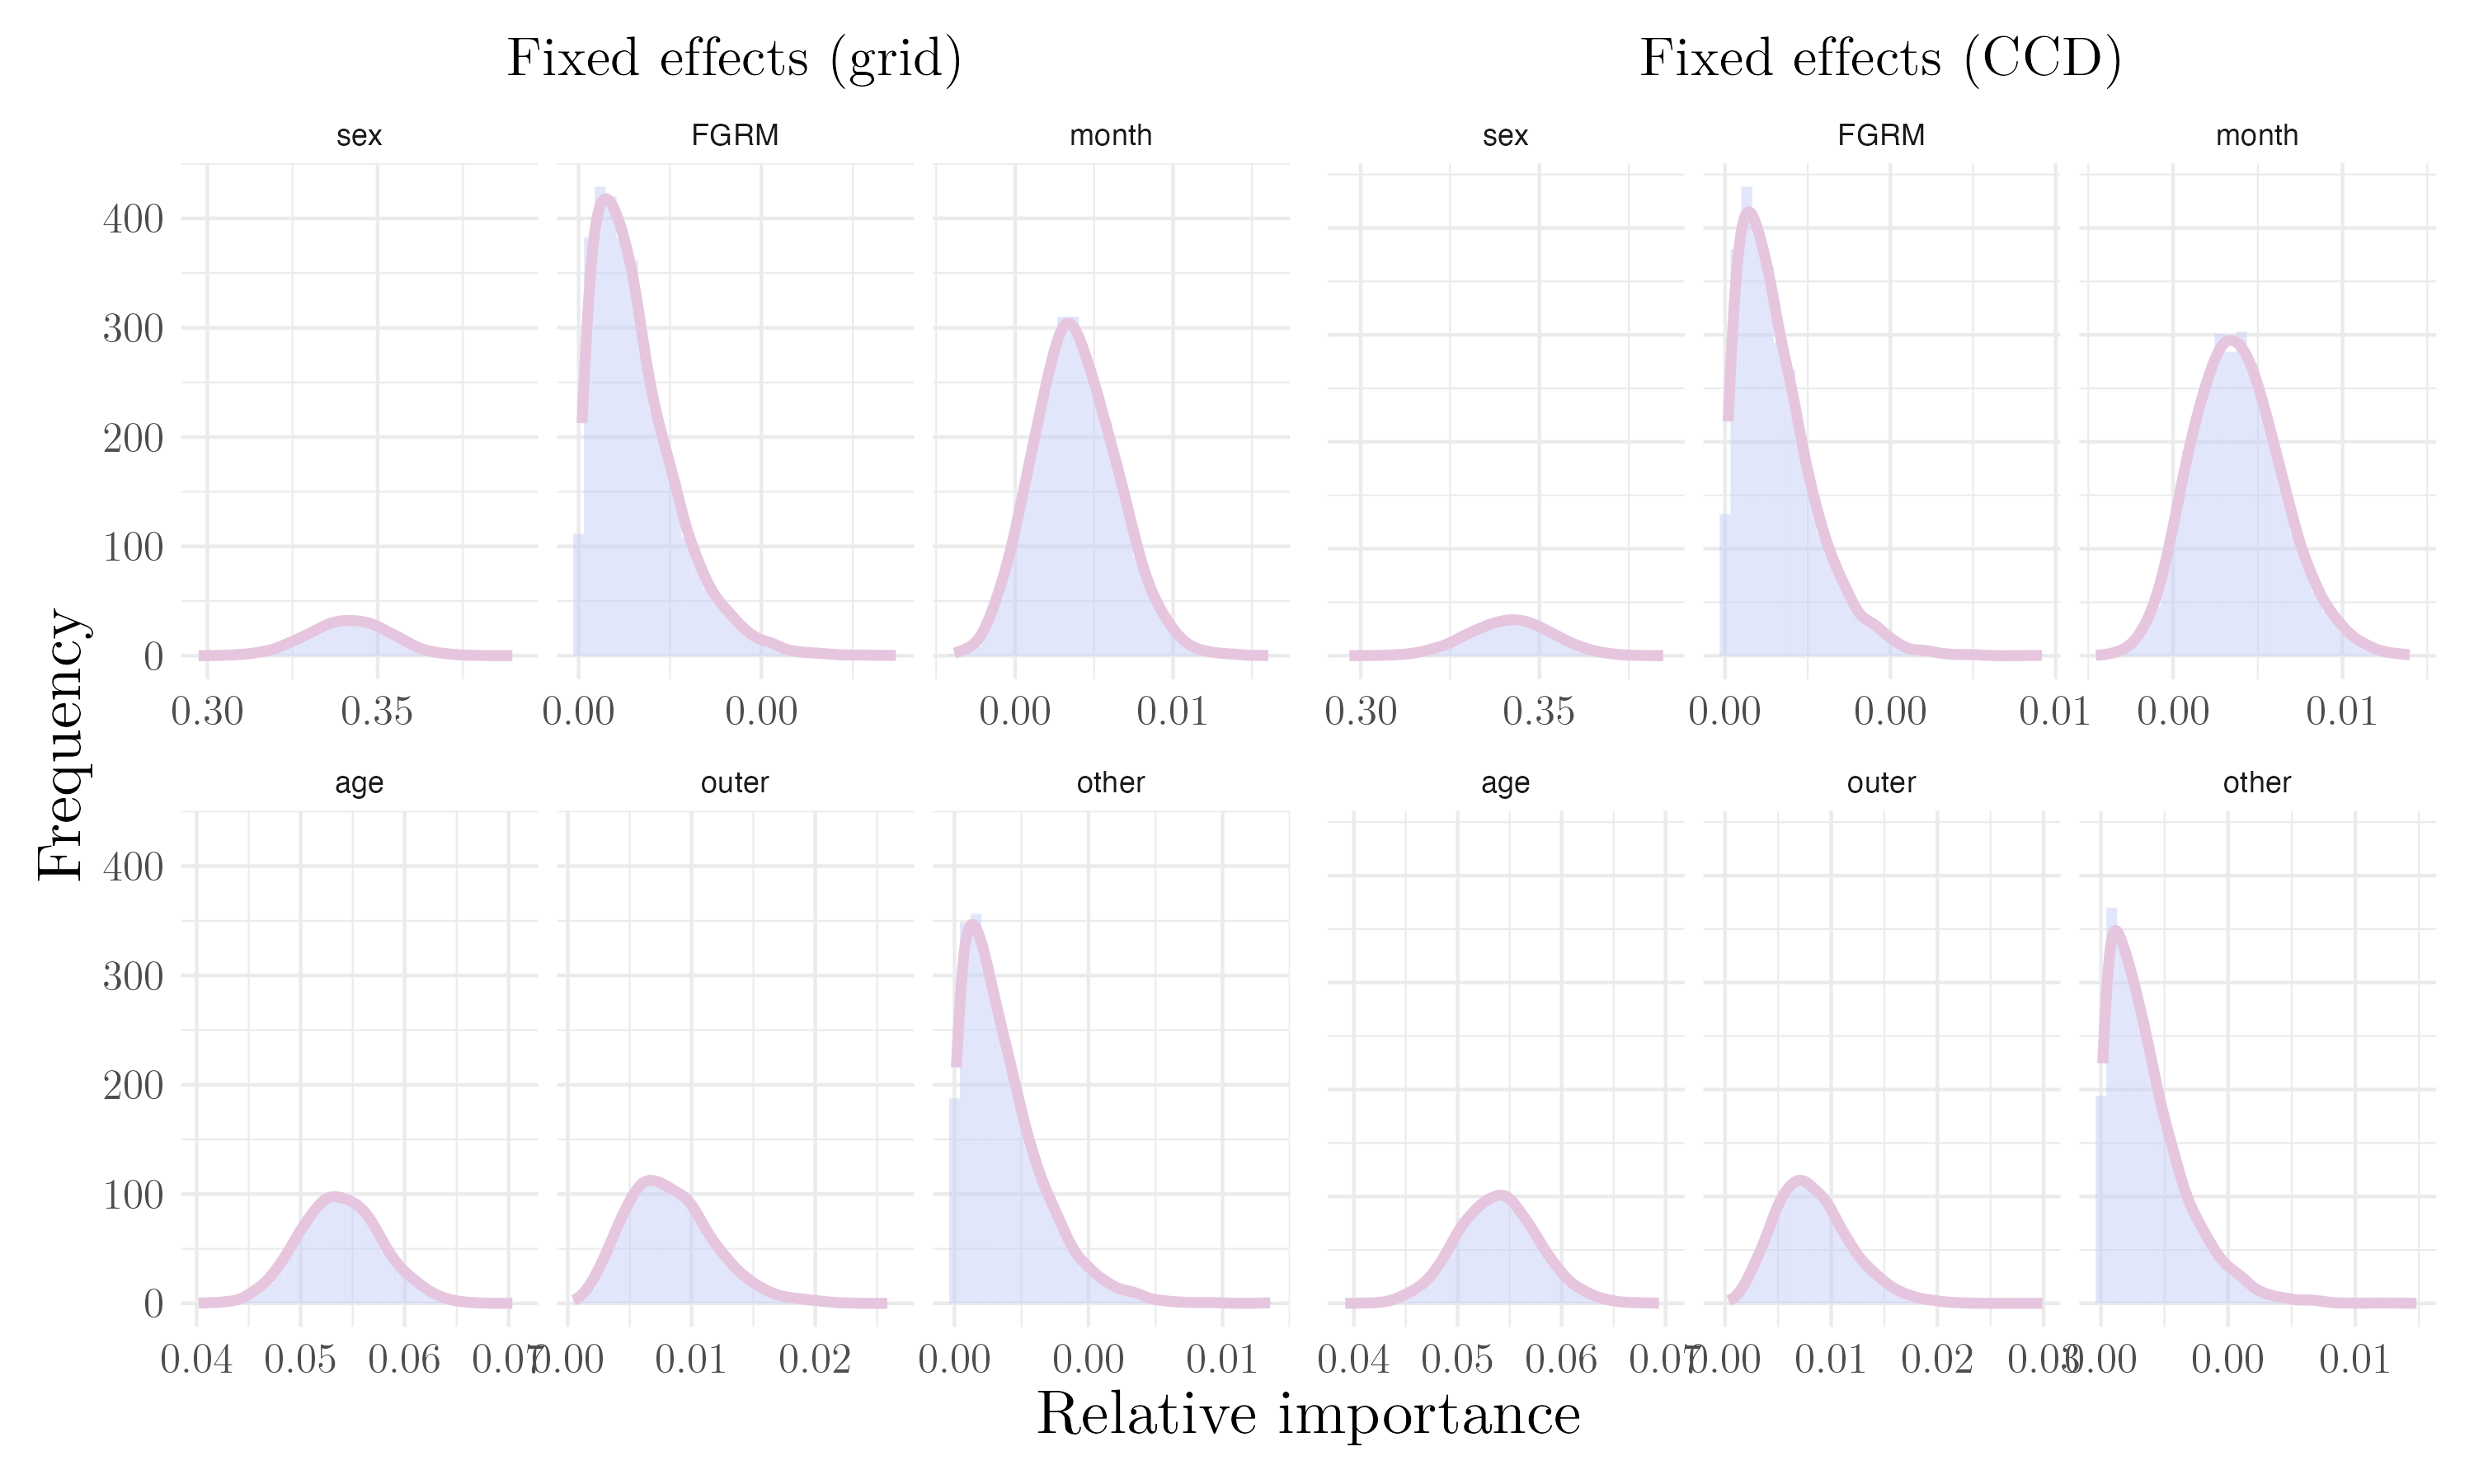
\includegraphics[width=1\linewidth]{Figures/House sparrow study/Wing_fixed.png}
  \caption[Posterior relative importance distributions of all fixed effects in wing length model for house sparrow study]{Posterior relative importance distributions of all fixed effects in wing length model for house sparrow study. The grid integration is displayed on the left, and CCD on the right.}
  \label{fig:wing_fixed_sparrows}
\end{figure}

\begin{figure}[H]%\ContinuedFloat
  \centering
  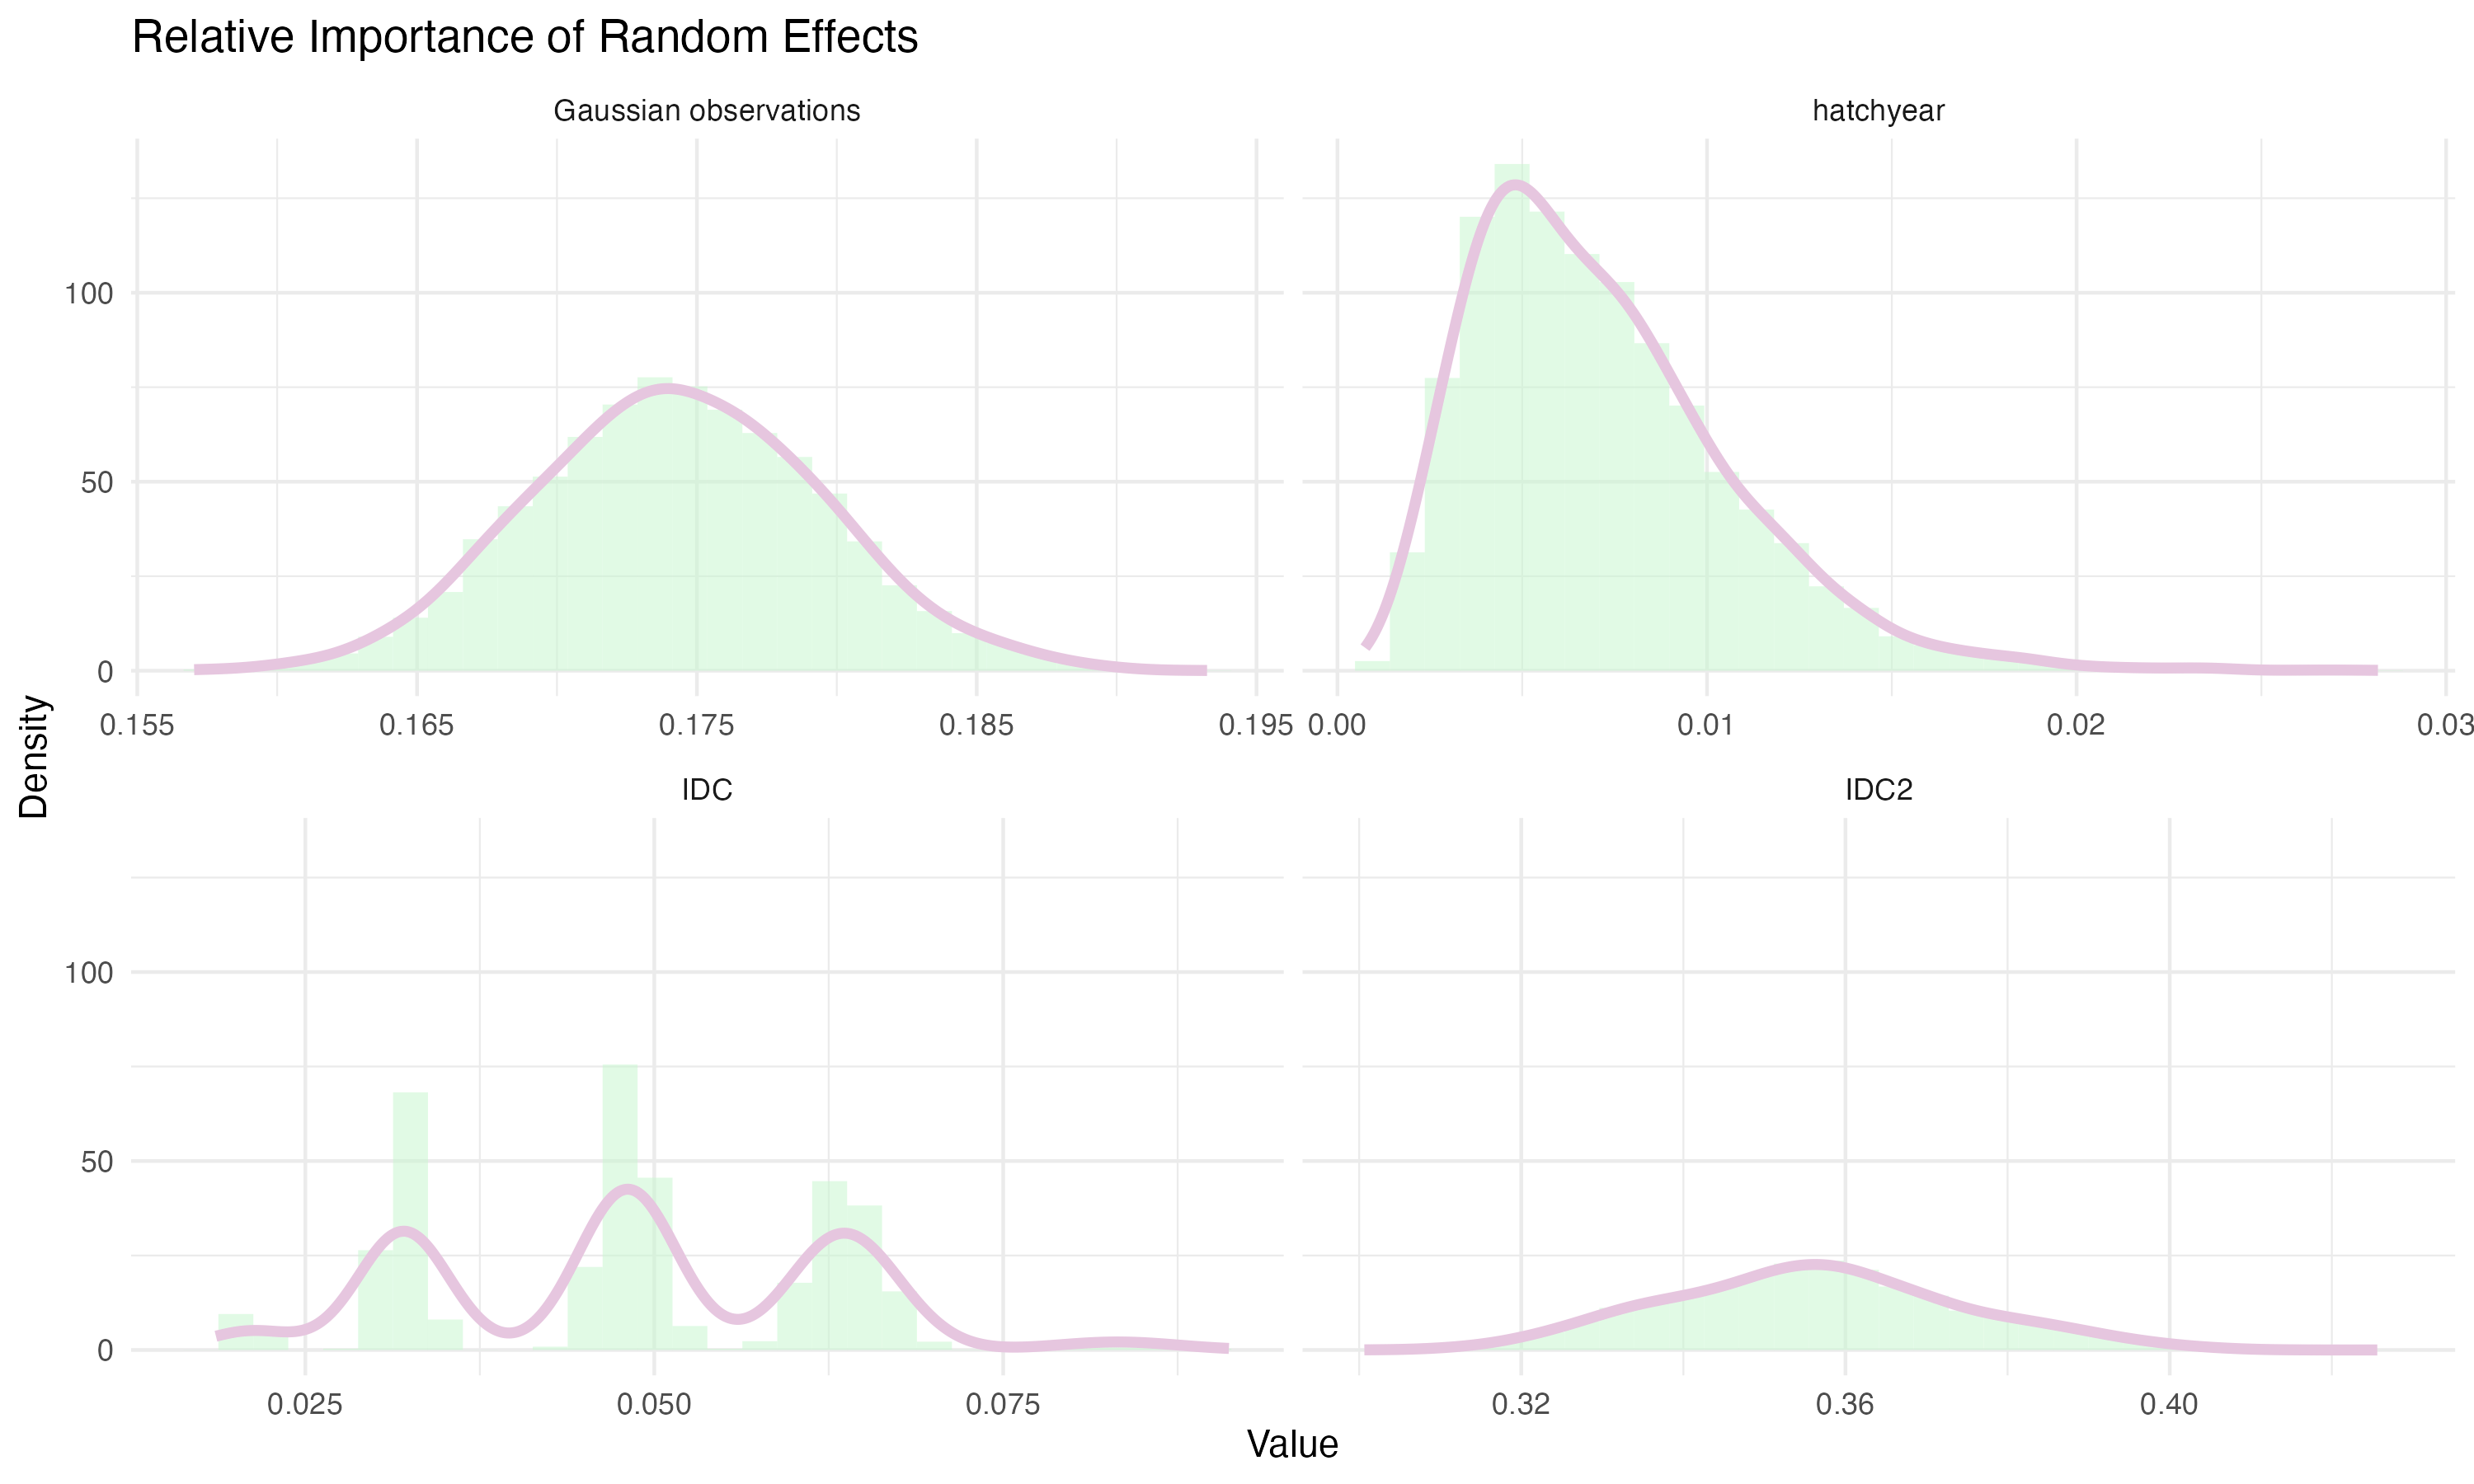
\includegraphics[width=1\linewidth]{Figures/House sparrow study/Wing_random.png}
  \caption[Posterior relative importance distributions of all random effects in wing length model for house sparrow study]{Posterior relative importance distributions of all random effects in heritability of wing length model for house sparrow study. The grid integration is displayed on the left, and CCD on the right.}
  \label{fig:wing_random_sparrows}
\end{figure}

\begin{figure}[H]%\ContinuedFloat
  \centering
  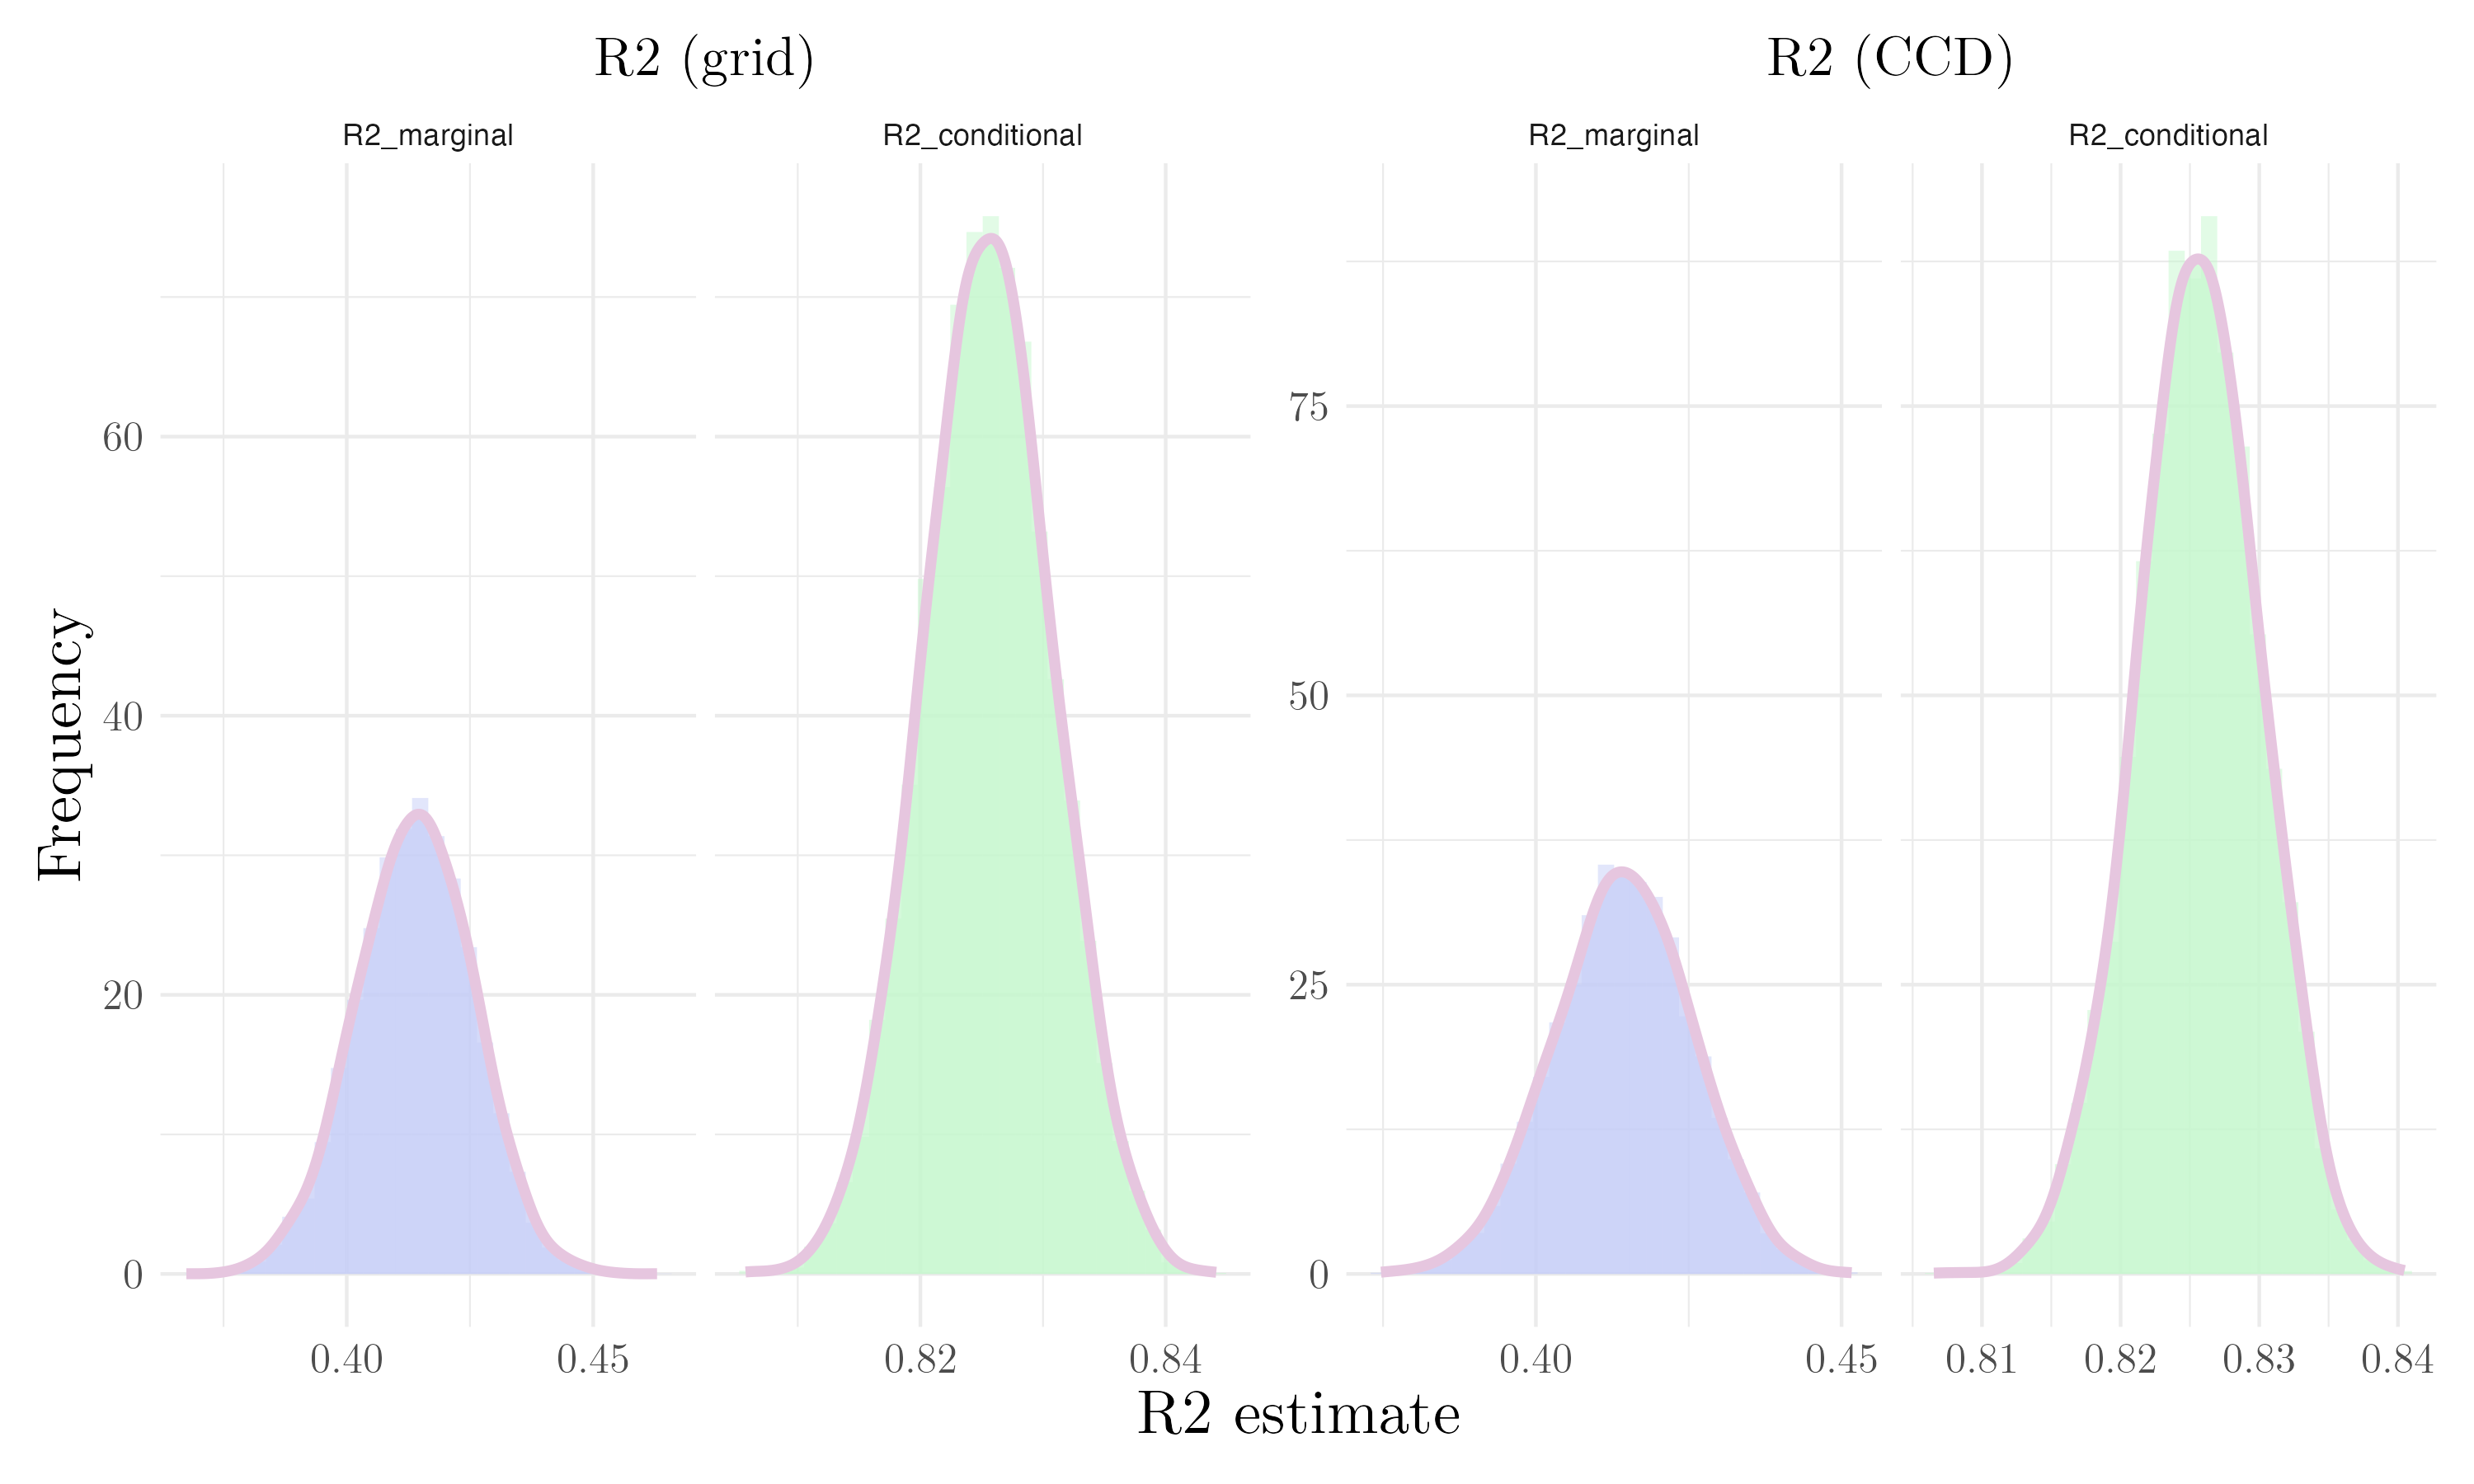
\includegraphics[width=1\linewidth]{Figures/House sparrow study/Wing_r2.png}
  \caption[Posterior distributions of $R^2$ values in wing length model for house sparrow study]{Posterior distributions of $R^2$ values in heritability of wing length model for house sparrow study. The grid integration is displayed on the left, and CCD on the right.}
  \label{fig:wing_r2}
\end{figure}

\begin{figure}[H]%\ContinuedFloat
  \centering
  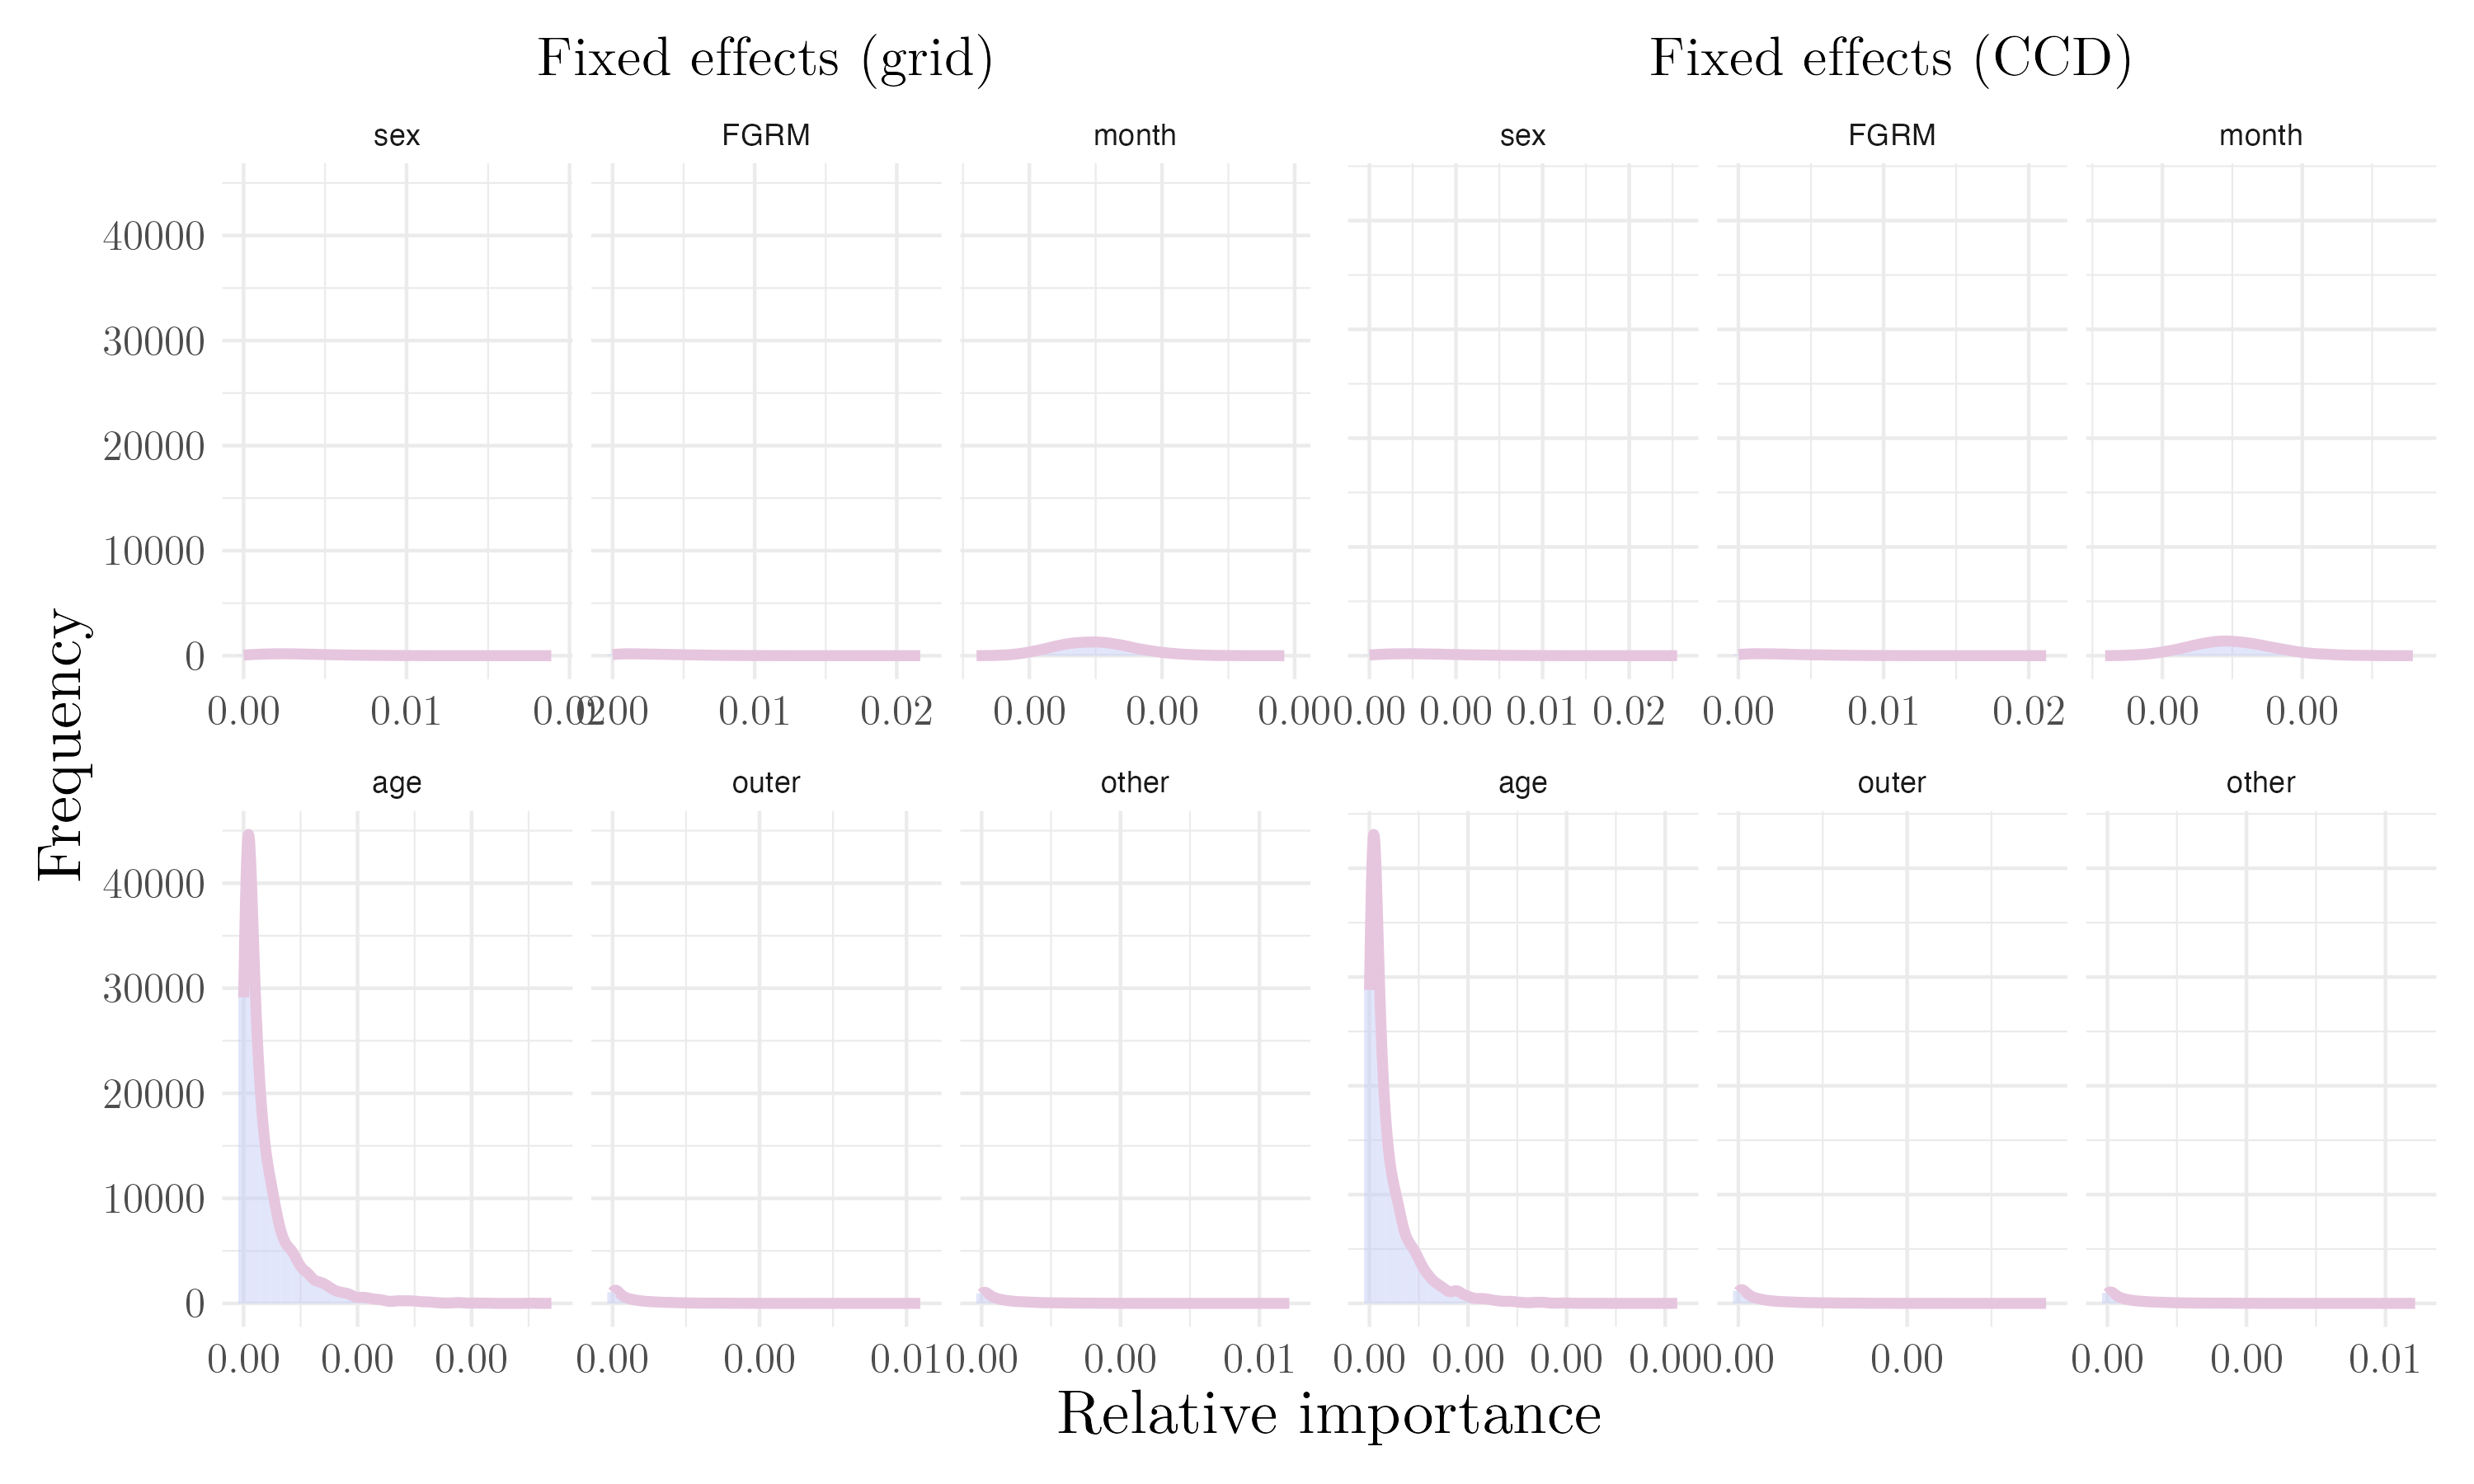
\includegraphics[width=1\linewidth]{Figures/House sparrow study/Tarsus_fixed.png}
  \caption[Posterior relative importance distributions of all fixed effects in tarsus length model for house sparrow study]{Posterior relative importance distributions of all fixed effects in heritability of tarsus length model for house sparrow study. The grid integration is displayed on the left, and CCD on the right.}
  \label{fig:tarsus_fixed_sparrows}
\end{figure}

\begin{figure}[H]%\ContinuedFloat
  \centering
  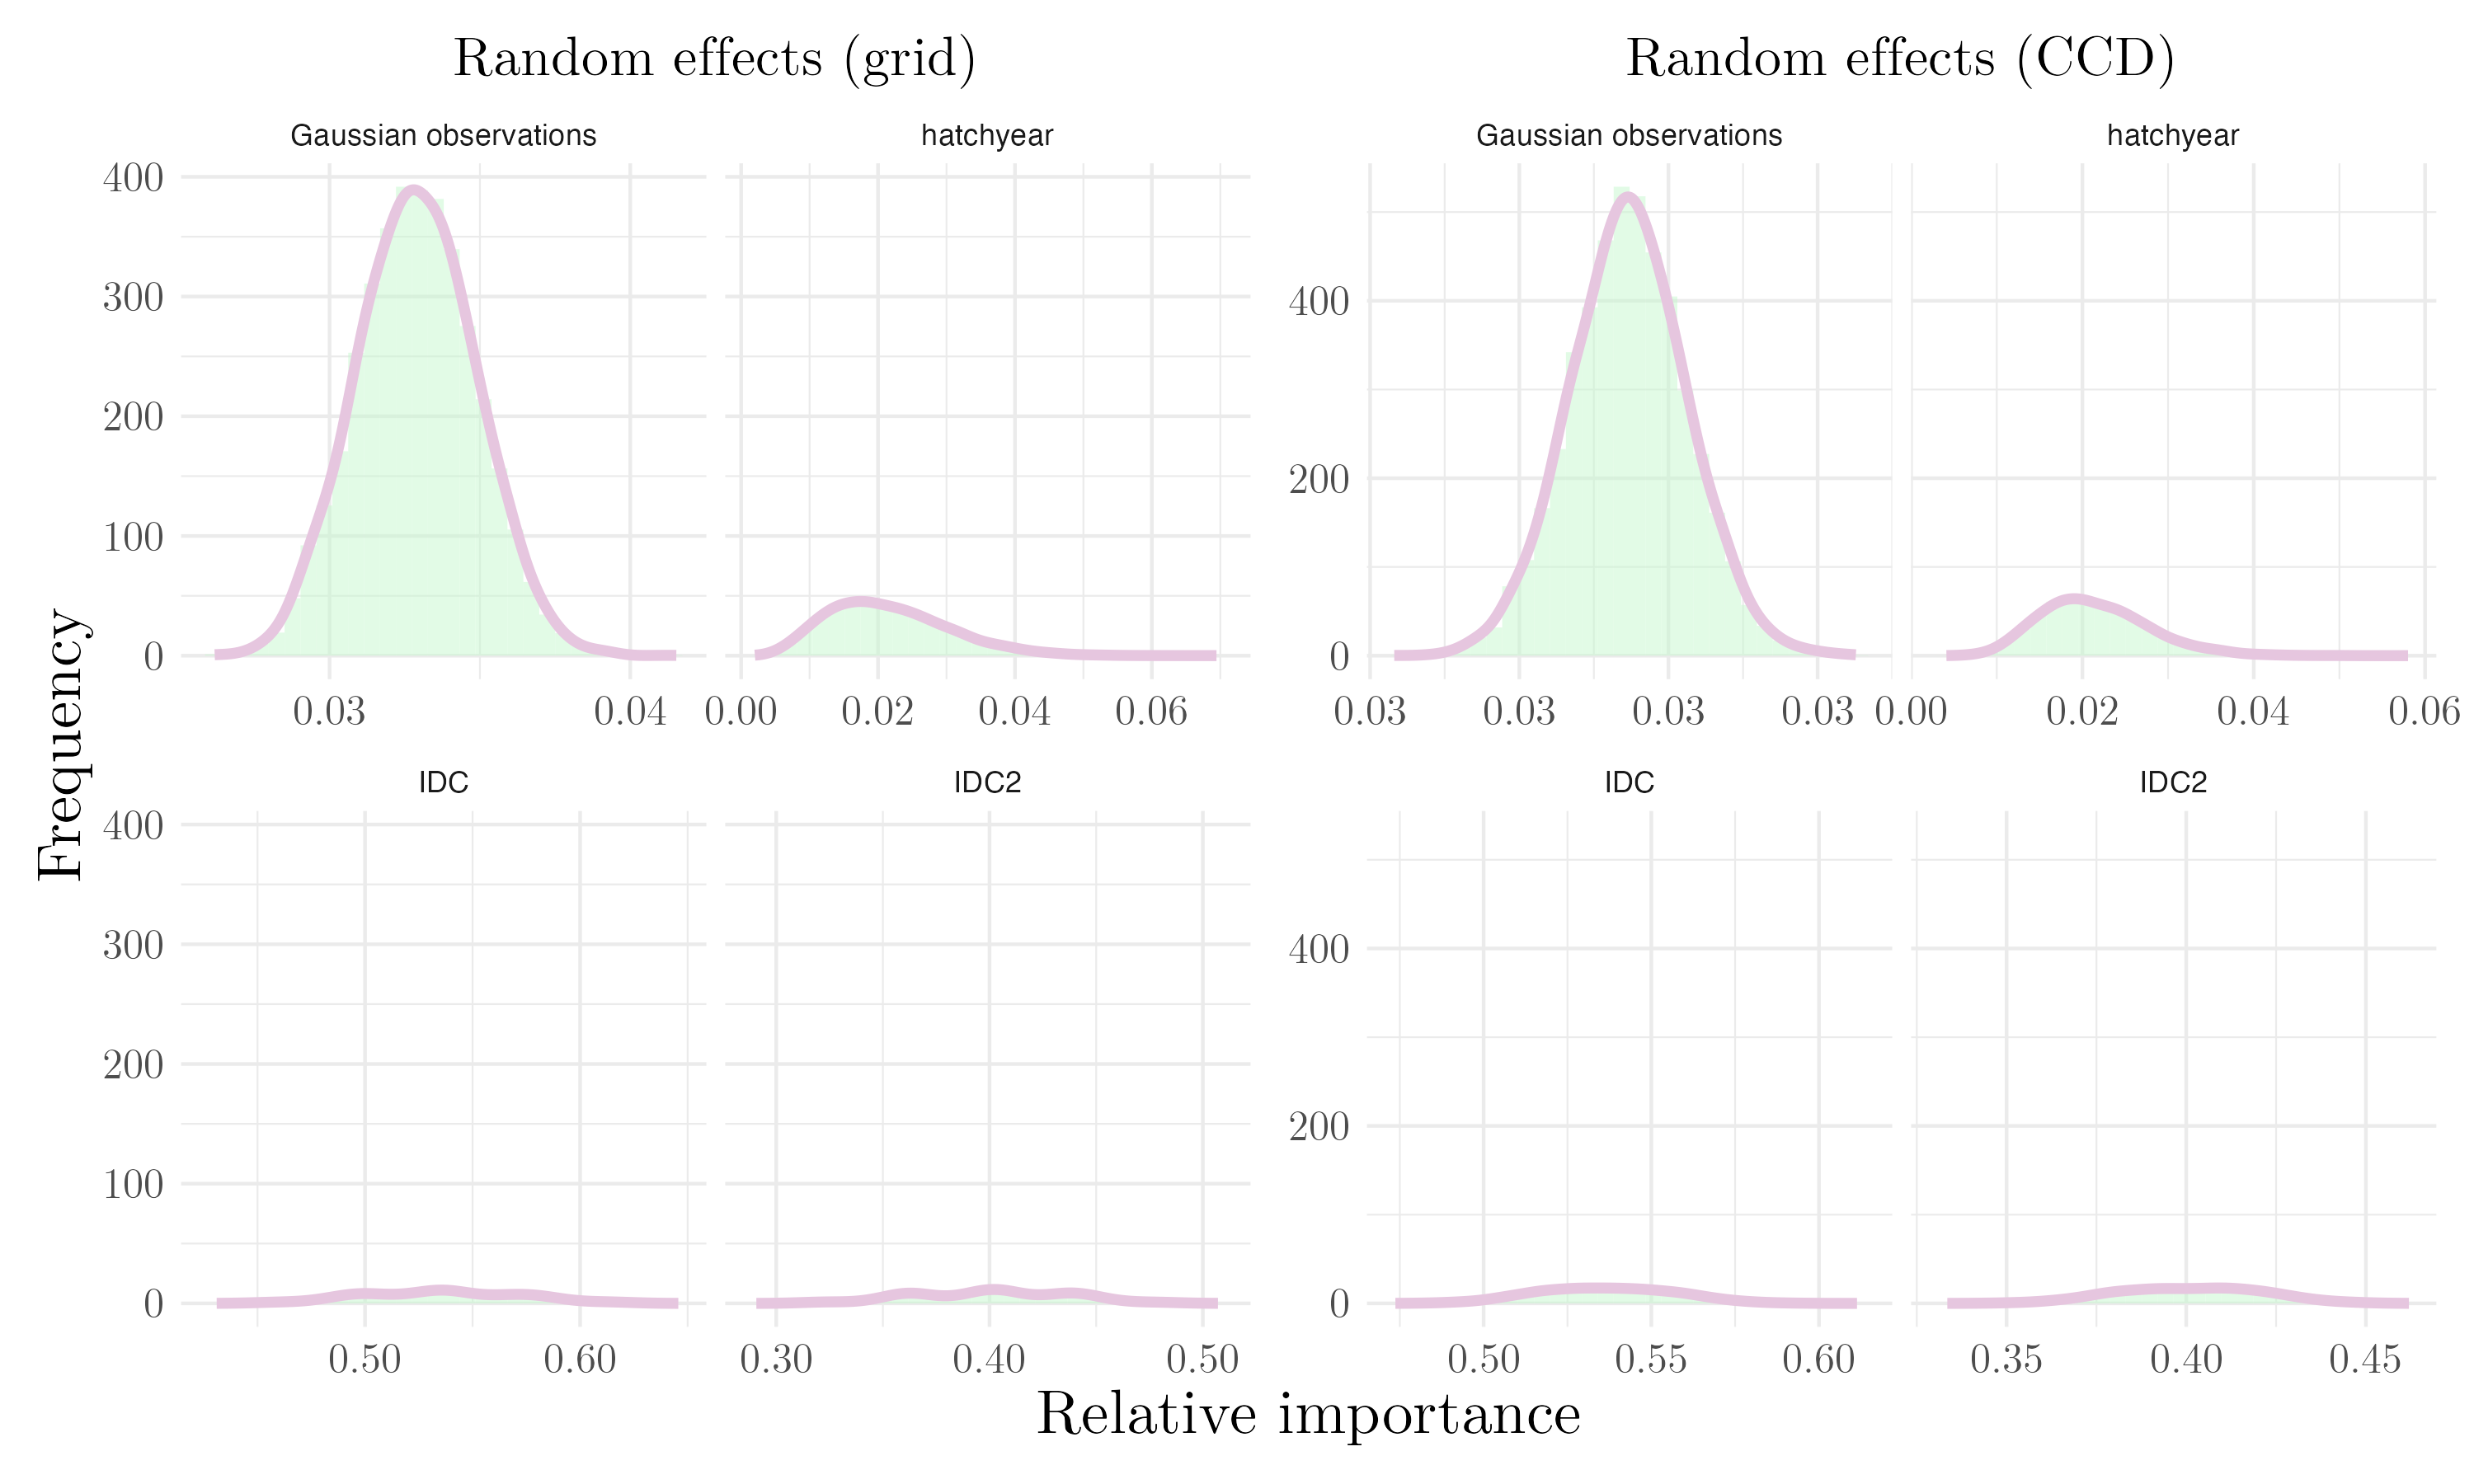
\includegraphics[width=1\linewidth]{Figures/House sparrow study/Tarsus_random.png}
  \caption[Posterior relative importance distributions of all random effects in tarsus length model for house sparrow study]{Posterior relative importance distributions of all random effects in heritability of tarsus length model for house sparrow study. The grid integration is displayed on the left, and CCD on the right.}
  \label{fig:tarsus_random_sparrows}
\end{figure}

\begin{figure}[H]%\ContinuedFloat
  \centering
  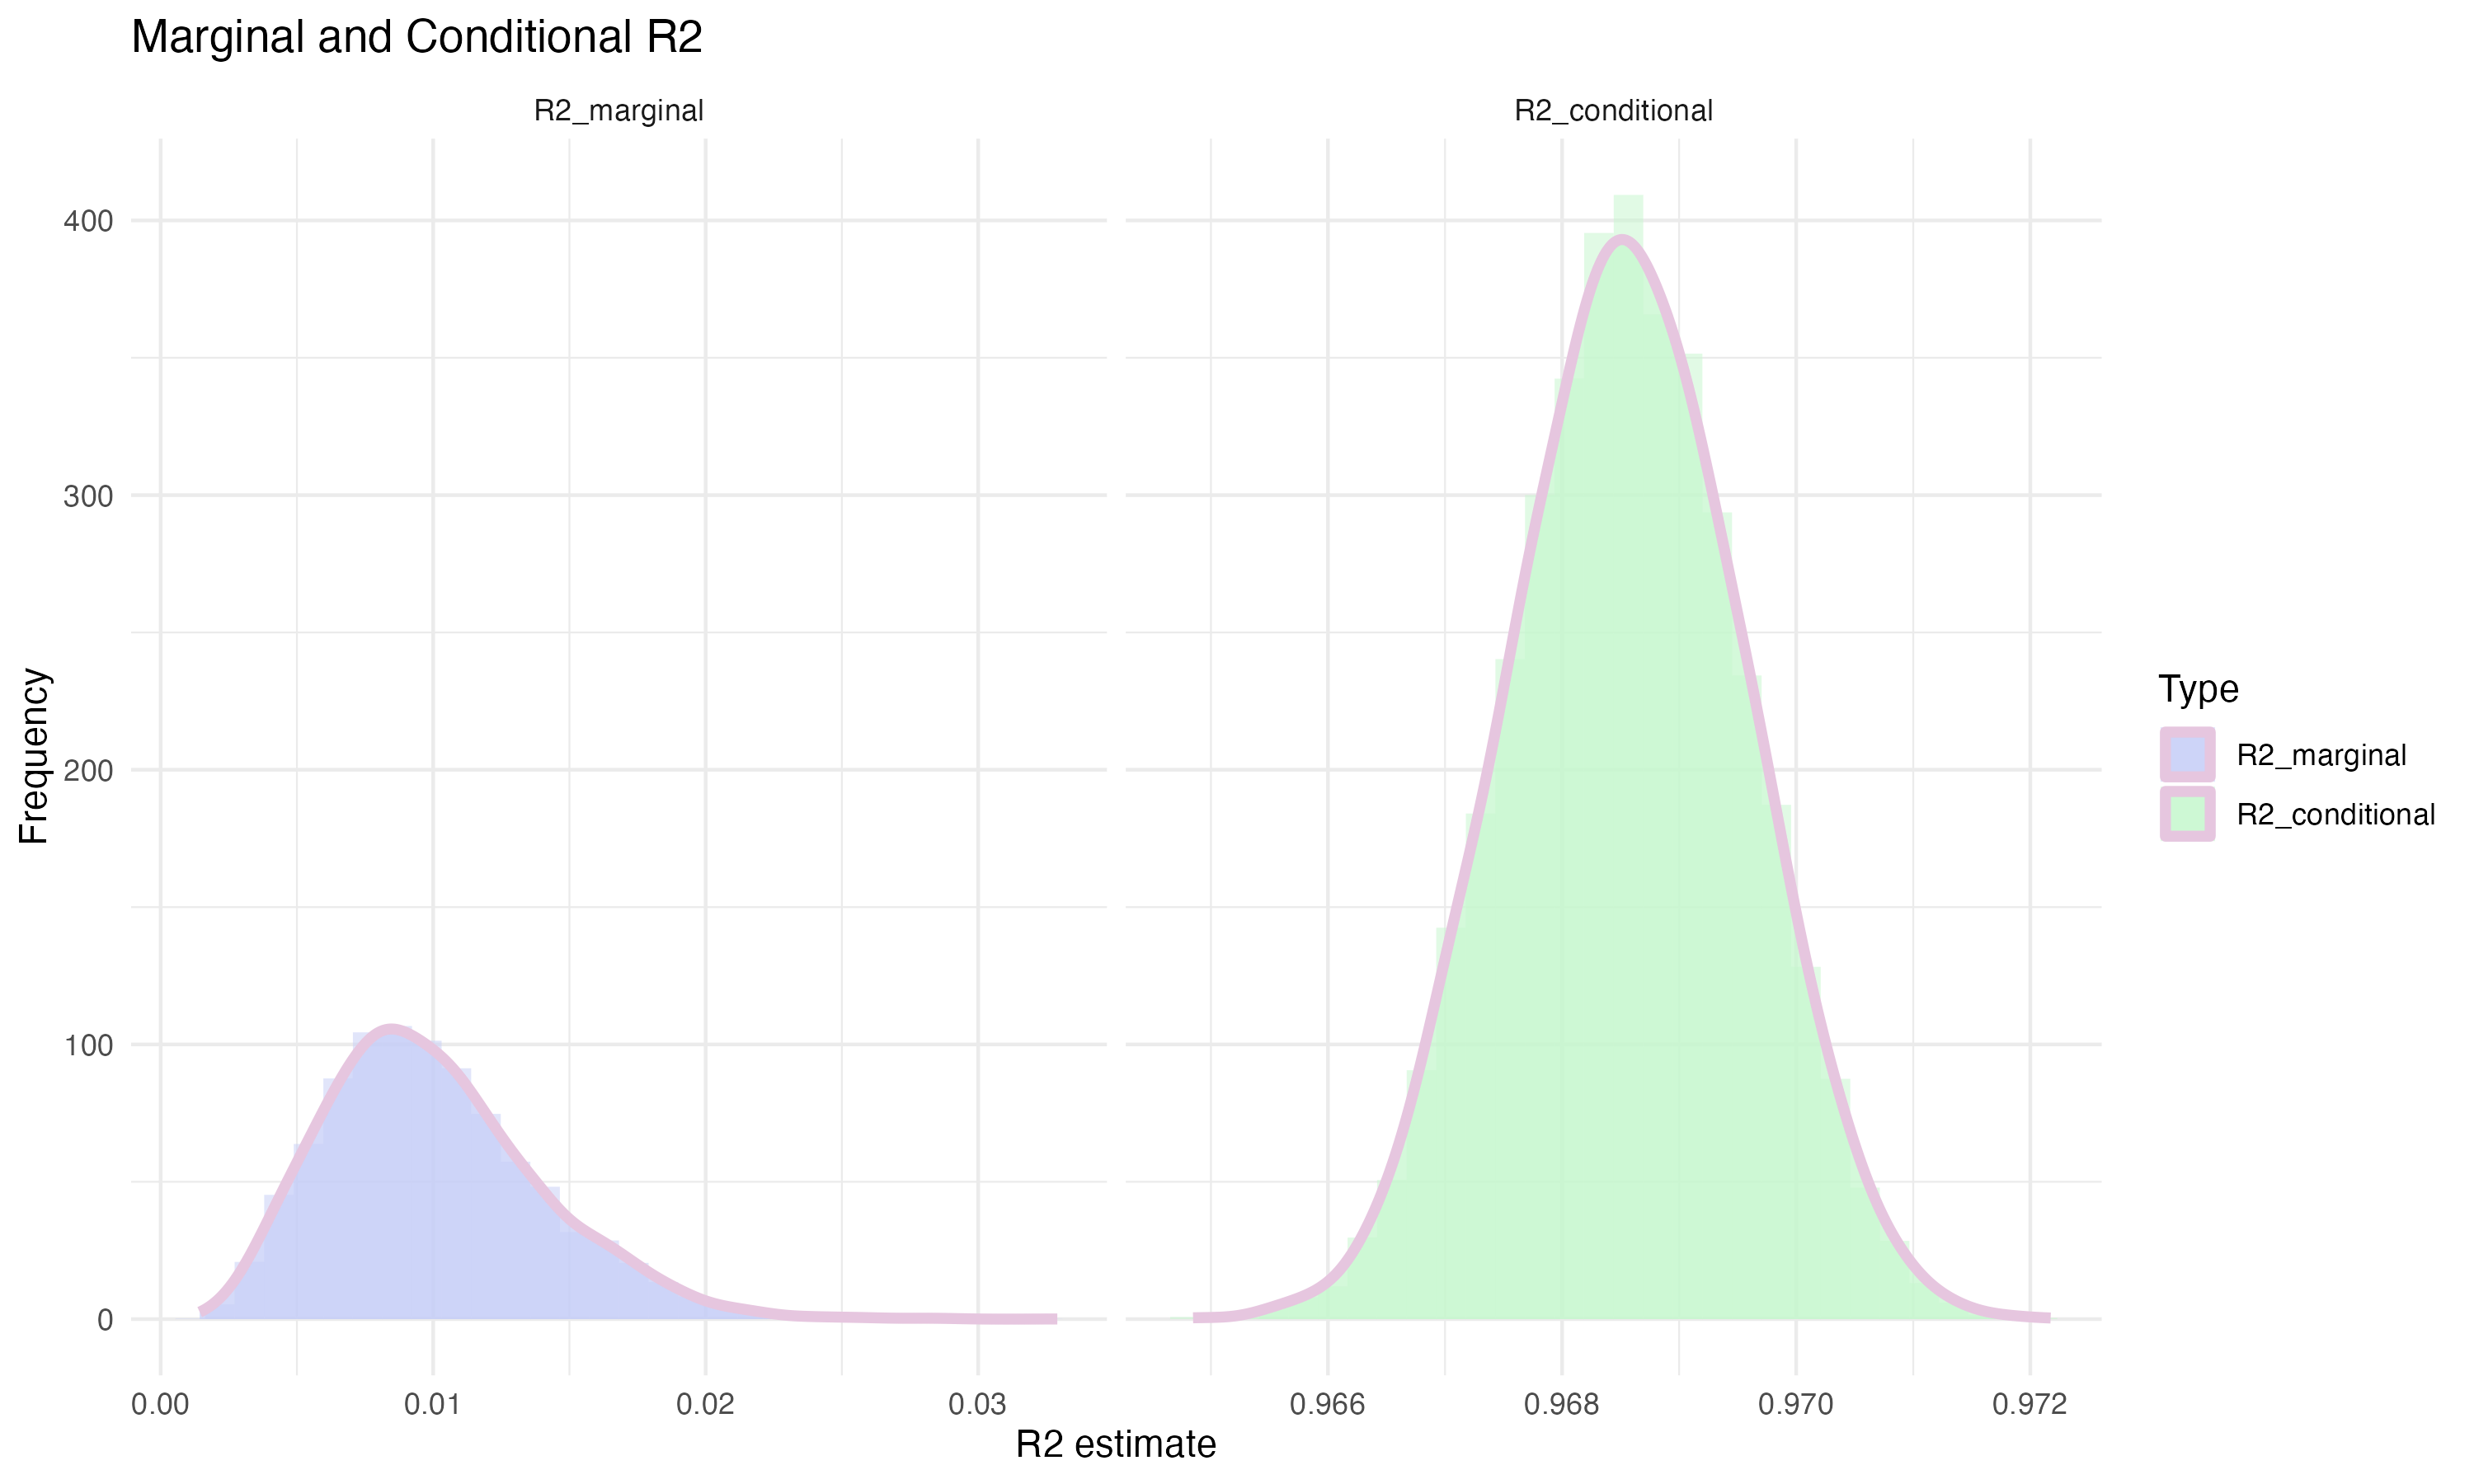
\includegraphics[width=1\linewidth]{Figures/House sparrow study/Tarsus_r2.png}
  \caption[Posterior distributions of $R^2$ values in tarsus length model for house sparrow study]{Posterior distributions of $R^2$ values in heritability tarsus length model for house sparrow study. The grid integration is displayed on the left, and CCD on the right.}
  \label{fig:tarsus_r2}
\end{figure}

\subsection*{Supplementary tables for the non-Gaussian simulation study}
We attach the summarizing tables for the Binomial and Poisson simulation studies here, as they were referred to throughout the thesis. Firstly, \Cref{table:summary_logit} contains summary statistics of the distribution obtained from the Binomial model, while \Cref{table:summary_poisson} contains the same for the Poisson model.

\begin{table}[!ht]
    \centering
    \begin{tabular}{@{}llcccccc@{}}
      \toprule
      \multicolumn{2}{c}{\textbf{Measure}} & $\mathbf{\rho=0}$ & $\mathbf{\rho=0.1}$ & $\mathbf{\rho=-0.1}$ & $\mathbf{\rho=0.4}$ & $\mathbf{\rho=-0.4}$ \\ \midrule
      \multirow{3}{*}{\shortstack{Relative Importance of \\ Random effect}} & Average & 0.0958 & 0.0859 & 0.1073 & 0.0674 & 0.1693 \\
                                         & 2.5\%   & 0.0687 & 0.0624 & 0.0794 & 0.0474 & 0.1304 \\
                                         & 97.5\%  & 0.1257 & 0.1118 & 0.1391 & 0.0891 & 0.2194 \\ \midrule
      \multirow{3}{*}{\shortstack{Relative Importance of \\ Fixed effect X1}} & Average & 0.0972 & 0.1169 & 0.0772 & 0.1732 & 0.0200 \\
                                           & 2.5\%   & 0.0802 & 0.1013 & 0.0628 & 0.1559 & 0.0165 \\
                                           & 97.5\%  & 0.1114 & 0.1333 & 0.0913 & 0.1902 & 0.0240 \\ \midrule
      \multirow{3}{*}{\shortstack{Relative Importance of \\ Fixed effect X2}} & Average & 0.1946 & 0.2097 & 0.1764 & 0.2387 & 0.0767 \\
                                           & 2.5\%   & 0.1738 & 0.1882 & 0.1557 & 0.2224 & 0.0638 \\
                                           & 97.5\%  & 0.2147 & 0.2321 & 0.1966 & 0.2570 & 0.0892 \\ \midrule
      \multirow{3}{*}{\shortstack{Relative Importance of \\ Fixed effect X3}} & Average & 0.2922 & 0.2984 & 0.2799 & 0.2984 & 0.1670 \\
                                           & 2.5\%   & 0.2674 & 0.2739 & 0.2551 & 0.2767 & 0.1462 \\
                                           & 97.5\%  & 0.3180 & 0.3208 & 0.3070 & 0.3177 & 0.1871 \\ \midrule
      \multirow{3}{*}{$R^2_m$}            & Average & 0.5839 & 0.6249 & 0.5336 & 0.7102 & 0.2637 \\
                                           & 2.5\%   & 0.5516 & 0.5935 & 0.5013 & 0.6835 & 0.2347 \\
                                           & 97.5\%  & 0.6143 & 0.6535 & 0.5653 & 0.7318 & 0.2900 \\ \midrule
      \multirow{3}{*}{$R^2_c$}            & Average & 0.6797 & 0.7108 & 0.6409 & 0.7776 & 0.4331 \\
                                           & 2.5\%   & 0.6526 & 0.6836 & 0.6126 & 0.7582 & 0.3919 \\
                                           & 97.5\%  & 0.7053 & 0.7352 & 0.6682 & 0.7973 & 0.4765 \\ \bottomrule
    \end{tabular}
    % \begin{tabular}{@{}llcccccc@{}}
    %   \toprule
    %   \multicolumn{2}{c}{\textbf{Measure}} & $\mathbf{\rho=0}$ & $\mathbf{\rho=0.1}$ & $\mathbf{\rho=-0.1}$ & $\mathbf{\rho=0.4}$ & $\mathbf{\rho=-0.4}$ \\ \midrule
    %   \multirow{3}{*}{\shortstack{Relative Importance of \\ Random effect}} & Average & 0.0947 & 0.0850 & 0.1079 & 0.0667 & 0.1694 \\
    %                                      & 2.5\%   & 0.0697 & 0.0609 & 0.0771 & 0.0488 & 0.1246 \\
    %                                      & 97.5\%  & 0.1223 & 0.1128 & 0.1420 & 0.0889 & 0.2153 \\ \midrule
    %   \multirow{3}{*}{\shortstack{Relative Importance of \\ Fixed effect X1}} & Average & 0.0978 & 0.1175 & 0.0774 & 0.1724 & 0.0200 \\
    %                                        & 2.5\%   & 0.0817 & 0.1025 & 0.0637 & 0.1580 & 0.0162 \\
    %                                        & 97.5\%  & 0.1134 & 0.1350 & 0.0917 & 0.1885 & 0.0245 \\ \midrule
    %   \multirow{3}{*}{\shortstack{Relative Importance of \\ Fixed effect X2}} & Average & 0.1951 & 0.2100 & 0.1763 & 0.2392 & 0.0769 \\
    %                                        & 2.5\%   & 0.1735 & 0.1903 & 0.1566 & 0.2206 & 0.0643 \\
    %                                        & 97.5\%  & 0.2155 & 0.2324 & 0.1956 & 0.2584 & 0.0911 \\ \midrule
    %   \multirow{3}{*}{\shortstack{Relative Importance of \\ Fixed effect X3}} & Average & 0.2922 & 0.2984 & 0.2795 & 0.2984 & 0.1666 \\
    %                                        & 2.5\%   & 0.2675 & 0.2742 & 0.2539 & 0.2770 & 0.1466 \\
    %                                        & 97.5\%  & 0.3187 & 0.3224 & 0.3047 & 0.3201 & 0.1909 \\ \midrule
    %   \multirow{3}{*}{$R^2_m$}            & Average & 0.5851 & 0.6258 & 0.5331 & 0.7100 & 0.2634 \\
    %                                        & 2.5\%   & 0.5549 & 0.5965 & 0.5023 & 0.6847 & 0.2357 \\
    %                                        & 97.5\%  & 0.6146 & 0.6552 & 0.5632 & 0.7360 & 0.2960 \\ \midrule
    %   \multirow{3}{*}{$R^2_c$}            & Average & 0.6799 & 0.7108 & 0.6411 & 0.7767 & 0.4328 \\
    %                                        & 2.5\%   & 0.6529 & 0.6865 & 0.6118 & 0.7555 & 0.3934 \\
    %                                        & 97.5\%  & 0.7046 & 0.7352 & 0.6677 & 0.7967 & 0.4729 \\ \bottomrule
    % \end{tabular}   
    \caption[Summary statistics for binomial GLMM simulation study]{Summary of simulation study results for the quantiles of relative importance estimates of the Logit model across different correlation levels. For $\rho=0$ the expected values are given in \Cref{table:3}.}
    \label{table:summary_logit}
\end{table}

\begin{table}[H]
    \centering
    \begin{tabular}{@{}llcccccc@{}}
      \toprule
      \multicolumn{2}{c}{\textbf{Measure}} & $\mathbf{\rho=0}$ & $\mathbf{\rho=0.1}$ & $\mathbf{\rho=-0.1}$ & $\mathbf{\rho=0.4}$ & $\mathbf{\rho=-0.4}$ \\ \midrule
      \multirow{3}{*}{\shortstack{Relative Importance of \\ Random effect}} & Average & 0.0953 & 0.0883 & 0.1043 & 0.0719 & 0.1465 \\
                                         & 2.5\%   & 0.0698 & 0.0663 & 0.0728 & 0.0525 & 0.1074 \\
                                         & 97.5\%  & 0.1235 & 0.1166 & 0.1366 & 0.0932 & 0.1940 \\ \midrule
      \multirow{3}{*}{\shortstack{Relative Importance of \\ Fixed effect X1}} & Average & 0.0969 & 0.1188 & 0.0751 & 0.1814 & 0.0170 \\
                                           & 2.5\%   & 0.0848 & 0.1064 & 0.0638 & 0.1708 & 0.0140 \\
                                           & 97.5\%  & 0.1075 & 0.1305 & 0.0857 & 0.1918 & 0.0205 \\ \midrule
      \multirow{3}{*}{\shortstack{Relative Importance of \\ Fixed effect X2}} & Average & 0.1940 & 0.2129 & 0.1712 & 0.2508 & 0.0657 \\
                                           & 2.5\%   & 0.1801 & 0.1987 & 0.1549 & 0.2400 & 0.0537 \\
                                           & 97.5\%  & 0.2096 & 0.2287 & 0.1872 & 0.2631 & 0.0791 \\ \midrule
      \multirow{3}{*}{\shortstack{Relative Importance of \\ Fixed effect X3}} & Average & 0.2917 & 0.3026 & 0.2725 & 0.3134 & 0.1420 \\
                                           & 2.5\%   & 0.2725 & 0.2848 & 0.2522 & 0.2994 & 0.1244 \\
                                           & 97.5\%  & 0.3102 & 0.3213 & 0.2925 & 0.3258 & 0.1615 \\ \midrule
      \multirow{3}{*}{$R^2_m$}            & Average & 0.5827 & 0.6343 & 0.5188 & 0.7456 & 0.2247 \\
                                           & 2.5\%   & 0.5570 & 0.6096 & 0.4937 & 0.7256 & 0.2009 \\
                                           & 97.5\%  & 0.6058 & 0.6570 & 0.5414 & 0.7650 & 0.2498 \\ \midrule
      \multirow{3}{*}{$R^2_c$}            & Average & 0.6780 & 0.7227 & 0.6231 & 0.8175 & 0.3712 \\
                                           & 2.5\%   & 0.6557 & 0.7020 & 0.5951 & 0.8032 & 0.3347 \\
                                           & 97.5\%  & 0.7001 & 0.7430 & 0.6476 & 0.8316 & 0.4141 \\ \bottomrule
    \end{tabular}
    % \begin{tabular}{@{}llcccccc@{}}
    %   \toprule
    %   \multicolumn{2}{c}{\textbf{Measure}} & $\mathbf{\rho=0}$ & $\mathbf{\rho=0.1}$ & $\mathbf{\rho=-0.1}$ & $\mathbf{\rho=0.4}$ & $\mathbf{\rho=-0.4}$ \\ \midrule
    %   \multirow{3}{*}{\shortstack{Relative Importance of \\ Random effect}} & Average & 0.0857 & 0.0781 & 0.0940 & 0.0627 & 0.1396 \\
    %                                      & 2.5\%   & 0.0642 & 0.0571 & 0.0679 & 0.0444 & 0.1002 \\
    %                                      & 97.5\%  & 0.1121 & 0.1023 & 0.1209 & 0.0809 & 0.1807 \\ \midrule
    %   \multirow{3}{*}{\shortstack{Relative Importance of \\ Fixed effect X1}} & Average & 0.0858 & 0.1045 & 0.0674 & 0.1579 & 0.0163 \\
    %                                        & 2.5\%   & 0.0751 & 0.0941 & 0.0582 & 0.1489 & 0.0138 \\
    %                                        & 97.5\%  & 0.0965 & 0.1149 & 0.0781 & 0.1671 & 0.0198 \\ \midrule
    %   \multirow{3}{*}{\shortstack{Relative Importance of \\ Fixed effect X2}} & Average & 0.1730 & 0.1874 & 0.1539 & 0.2192 & 0.0627 \\
    %                                        & 2.5\%   & 0.1594 & 0.1754 & 0.1395 & 0.2086 & 0.0525 \\
    %                                        & 97.5\%  & 0.1873 & 0.2006 & 0.1697 & 0.2301 & 0.0743 \\ \midrule
    %   \multirow{3}{*}{\shortstack{Relative Importance of \\ Fixed effect X3}} & Average & 0.2588 & 0.2677 & 0.2447 & 0.2740 & 0.1357 \\
    %                                        & 2.5\%   & 0.2423 & 0.2524 & 0.2277 & 0.2617 & 0.1197 \\
    %                                        & 97.5\%  & 0.2757 & 0.2831 & 0.2638 & 0.2851 & 0.1529 \\ \midrule
    %   \multirow{3}{*}{$R^2_m$}            & Average & 0.5176 & 0.5596 & 0.4660 & 0.6510 & 0.2147 \\
    %                                        & 2.5\%   & 0.4978 & 0.5377 & 0.4463 & 0.6339 & 0.1936 \\
    %                                        & 97.5\%  & 0.5355 & 0.5783 & 0.4878 & 0.6679 & 0.2361 \\ \midrule
    %   \multirow{3}{*}{$R^2_c$}            & Average & 0.6033 & 0.6378 & 0.5600 & 0.7138 & 0.3543 \\
    %                                        & 2.5\%   & 0.5815 & 0.6197 & 0.5350 & 0.6962 & 0.3181 \\
    %                                        & 97.5\%  & 0.6245 & 0.6597 & 0.5848 & 0.7290 & 0.3900 \\ \bottomrule
    % \end{tabular}
    \caption[Summary statistics for Poisson GLMM simulation study]{Summary of simulation study results for the quantiles of relative importance estimates the Poisson model across different correlation levels. For $\rho=0$ the expected values are given in \Cref{table:3}.}
    \label{table:summary_poisson}
  \end{table}
